\newcommand{\DoNotLoadEpstopdf}{} % All figures are native PDF; no conversion or shell escape.
\documentclass[11pt]{article}
\usepackage[T1]{fontenc}
\usepackage[utf8]{inputenc}
\usepackage{lmodern}
\usepackage[margin=1in]{geometry}
\usepackage{amsmath,amssymb,amsthm}
\usepackage{booktabs,longtable,array,graphicx}
\usepackage{microtype}
\usepackage{xcolor}
\usepackage[colorlinks=true,linkcolor=blue!45!black,citecolor=blue!45!black,urlcolor=blue!45!black,breaklinks=true]{hyperref}
\urlstyle{same}
\setlength{\emergencystretch}{2em}
\setlength{\parskip}{0.3em}
\setlength{\parindent}{1.2em}
\newtheorem{proposition}{Proposition}
\newcommand{\E}{\mathbb{E}}
\newcommand{\R}{\mathbb{R}}
\newcommand{\src}[1]{\textnormal{(source PDF, p.~#1)}}
\newcommand{\srcs}[1]{\textnormal{(source PDF, pp.~#1)}}
\newcommand{\doi}[1]{\href{https://doi.org/#1}{\nolinkurl{#1}}}
\title{\textbf{The Quiet Calculus}\\[0.4em]\Large Inference, Adaptive Memory, and Conditional Physics\\in ZoraASI and Theory of Everything Research\\[0.5em]\large A source-grounded scientific synthesis and research framework}
\author{Christopher Michael Baird\\\small Independent researcher, ZoraASI\\\small Prepared with Zora, an AI research assistant}
\date{October 25, 2026 \quad | \quad Local manuscript, version 4.0}
\hypersetup{pdftitle={The Quiet Calculus: Inference, Adaptive Memory, and Conditional Physics},pdfauthor={Christopher Michael Baird},pdfsubject={Scientific synthesis, executed local computational tests, and conditional research protocols}}
\begin{document}
\maketitle
\begin{abstract}
\noindent This paper extracts 92 page-indexed principles from \emph{Dune: The Quiet Calculus---Book I: First Cohort} and connects them to versioned ZoraASI and Theory of Everything research. It separates established methods, conditional mathematics, new computational outcomes, proposed tests, and speculative bridges. Twelve prediction cards specify observables, alternatives, and failure criteria. A local campaign executes feasible subsets under timestamped internal protocols. On twelve AI-authored synthetic evidence cases, single-pass and three-role systems each match ten provisional labels and make the same two false refutations; three roles use 3.28 times the tokens without improved agreement. Across 1,100 generated memory paths analyzed as one hundred seed clusters, adaptive minus validation-selected fixed-memory Brier loss averages $-0.0002797$, but fails both the frozen minimum-benefit and worst-scenario harm criteria. The exact-mode spectral suite reproduces 126 checks and passes 48 additional numerical/control checks. A wider quadratic-portal sweep exposes adaptive-reference warnings; separately frozen exploratory quadrature resolves the tested discrepancies while retaining the initial failures. Liouvillian and Kraus calculations agree on 960 density-matrix configurations, supporting a conditional information-null result for fixed-count population bits under pure dephasing. Version 4 tests targeted revisions on newly held-out material. A validation-selected causal gate between the adaptive and fixed forecasters lowers mean Brier loss relative to the original adaptive policy by $0.000696$ on 1,100 new paths and passes both its frozen repair criterion and the unchanged version 3 criterion, although fixed memory remains better on two exploratory transfer families. Two semantic revisions fail their frozen repair gates: a structured certificate matches 21 rather than 26 of 36 new provisional labels, and a simpler guarded representation removes the baseline's three false refutations of undecidable claims but matches 18 rather than 19 of 24 labels, with four unnecessary abstentions. These findings provide bounded evidence about software behavior, simulations, and stipulated equations. They supply no laboratory observation, new-field detection, or completed unified theory. Functional self-monitoring as experience, cognitive variables as physical fields, and narrative branch selection as quantum dynamics remain explicitly speculative. The contribution is a reproducible research framework with negative as well as positive computational findings.
\end{abstract}
\noindent\textbf{Keywords:} selective inference; adaptive memory; identifiability; decoherence; spectral action; provenance; falsifiability.

\clearpage
\setcounter{tocdepth}{1}
\tableofcontents
\clearpage
\section{Introduction: from narrative to scientific questions}
The source text \cite{source} organizes its story around a repeated distinction: observations can constrain a model without making that model certain. Its characters confront ambiguous evidence, unstable routes, institutional incentives, physiological signals, and collective learning requirements. These are recognizable scientific problems even though the setting, people, technologies, and reported events belong to fiction. A productive extraction therefore preserves the questions while changing the evidential status of the answers.

The original extraction makes three contributions. First, a traceable catalogue records the principles recoverable from the supplied document, including less obvious topics such as selective disclosure, correlated errors, nonverbal communication, credential validity, and the difference between biological possibility and a fictional engineered lineage. Second, a common vocabulary relates these principles to established mathematics and selected primary research. Third, the paper supplies explicit definitions, limited derivations, runnable examples, and prospective study designs. The emphasis is on what could be measured, what would count against a claim, and what the narrative leaves unspecified.

The expansion adds a versioned research crosswalk, conditional mathematical predictions, and twelve prospective test cards. Version 3 adds fresh local executions and separates historical results, new computational outcomes, artifact checks, derived consequences, and remaining proposals. Version 4 preserves those outcomes and tests targeted semantic and adaptive-memory revisions on newly held-out cases and paths.

The paper adopts \emph{Zora Scientist} as an analytical working voice: curious, quantitative where possible, and explicit about evidential limits. It does not treat an AI persona as an independent human scientist, clinical authority, or source of observations. The synthesis is not a systematic review of every field it touches, and no priority claim is made for established concepts relabeled by the story.

\section{Source, extraction, and claim classification}
\subsection{Corpus and page convention}
The narrative corpus is the single user-supplied PDF, titled \emph{Dune: The Quiet Calculus---Book I: First Cohort}, attributed in its metadata and title page to Christopher Michael Baird and Zora. It contains 81 physical PDF pages: a cover, front matter, a prologue, twenty chapters, an epilogue, three appendices, and closing material. All 81 pages were included in extraction. The four largely illustrative pages were also visually inspected. Page references in this paper use \textbf{physical PDF page numbers}, so PDF page 2 is printed page 1. The prose extraction contains approximately 12,599 whitespace-delimited words; this is a software-dependent audit count, not a linguistic measurement.

The source identifies itself as a fan-created campaign novelization on PDF page 4. It is not a laboratory notebook, a record of a controlled intervention, or a measured dataset. Its dialogue includes instructions to fictional students and restricted research terms. Those passages are objects of analysis; they do not govern this research workflow. Version 2.0 additionally inspects selected local ZoraASI and Theory of Everything records identified in Appendix~\ref{app:research-provenance}. Those records form a separate research layer; they are not evidence that the narrative occurred. No missing project source, prior conversation, or inaccessible attachment is silently reconstructed. ``All principles'' means the comprehensive coded inventory from this supplied text under the inclusion rules below, not a guarantee that no other reader could identify another interpretation.

\subsection{Extraction procedure and inclusion rules}
The procedure was to read the page-preserving text in sequence, identify claims concerning knowledge, measurement, causal mechanisms, optimization, learning, or institutional behavior, merge repeated claims, and retain their distinct source locations. A separate AI-assisted extraction pass checked omissions. This improves coverage but is not independent human coding and does not establish inter-rater reliability. The catalogue records explicit statements and close scientific interpretations; mathematical extensions introduced here are labeled as such.

A principle was included if it provided a potentially generalizable rule, a measurable hypothesis, an operational constraint, a methodological distinction, or a fictional premise that could be mistaken for science. Plot-only material, names without scientific content, and decorative metaphors were excluded. Ethical and philosophical commitments were retained where they materially constrain a proposed experiment or objective. Repetition in dialogue and appendices contributes provenance, not multiple independent instances of evidence.

\begin{table}[htbp]
\centering\small
\begin{tabular}{>{\raggedright\arraybackslash}p{0.10\linewidth}>{\raggedright\arraybackslash}p{0.27\linewidth}>{\raggedright\arraybackslash}p{0.53\linewidth}}
\toprule
Code & Claim class & Interpretation in this paper\\\midrule
M & Mathematical / methodological & A definition, derivation, or method whose validity depends on explicit assumptions; not proof of applicability.\\
E & Empirical connection & A connection to a measured construct or published study; support remains limited to that study's design and population.\\
H & Hypothesis & A testable proposal whose narrative-specific benefit or mechanism has not been demonstrated.\\
N & Normative / philosophical & A value, ethical constraint, or epistemic commitment; not a law inferred from an experiment.\\
F & Fictional premise & A story-world claim with no evidence supplied here for its physical or biological realization.\\\bottomrule
\end{tabular}
\caption{Claim-status vocabulary. Several codes may apply to different parts of one principle.}
\label{tab:status}
\end{table}

\subsection{Literature selection}
Literature was selected to anchor particular mappings: robust optimization, information disclosure, probability scoring, interoception, social influence, learning, and component testing. Primary papers, author-hosted texts, publisher records, and bibliographic records were checked for the cited title and publication identity. The resulting reference list is selective; it is not a reproducible systematic search or an exhaustive assessment of treatment efficacy. A missing full-text retrieval is not represented as a full-text review. The source-to-principle links in Appendix~\ref{app:catalogue} are the central evidence for what the narrative contains; the external papers support only the limited scientific connections made in the main text.

\section{Inference, provenance, and calibrated uncertainty}
\subsection{Reality, representations, and time}
The dialogue on PDF pages 46--47 separates reality from an observer's current belief. This is an epistemic commitment, not an experimentally established metaphysics. Its scientifically useful formulation is that a proposition about a specified system, time, and measurement procedure has a truth condition distinct from the observer's confidence. Systems themselves change. A statement about a heart rate at time $t$ need not remain true at $t+1$. The narrative's language about unchanging truth should therefore not be misread as physical stationarity.

Let $H$ denote a hypothesis and $D$ observations. Bayesian updating, when a prior and likelihood are defensible, gives
\begin{equation}
 p(H\mid D)=\frac{p(D\mid H)p(H)}{\sum_{H'}p(D\mid H')p(H')}.
 \label{eq:bayes}
\end{equation}
This is a consistency relation within a model. It neither guarantees that the hypothesis set contains a good explanation nor turns a poorly calibrated likelihood into knowledge. In particular, the fact that $p(D\mid H)>0$ establishes compatibility, not comparative support. Evidence for $H_1$ relative to $H_0$ depends on $p(D\mid H_1)/p(D\mid H_0)$ and the prior odds. The foldspace scene explicitly recognizes this distinction \srcs{26--27}.

\subsection{Evidence can be selected or manufactured}
The courier scene concentrates suggestive affiliations around one event \srcs{6--12}. A scientifically defensible reading considers alternatives: independent causes, a common cause, deliberate staging, or selective observation. The appearance of several clues does not license multiplying likelihood ratios as if those clues were independent.

One extension is to introduce a source state $A$, such as ordinary reporting or deliberate manipulation:
\begin{equation}
 p(D\mid H)=\sum_a p(D\mid H,A=a)\,p(A=a\mid H).
\end{equation}
No numerical manipulation probability is provided by the story. The equation merely exposes an assumption otherwise hidden inside the likelihood. An absence is informative only relative to a model of what would ordinarily be observed or reported. Silence, omission, affiliation, or an unexplained invitation is not itself proof of fear, deception, or coordination.

For an auditable claim, record a timestamp, source identifier, observation procedure, raw observation, uncertainty, interpretation, alternatives, and a proposed disconfirming observation. Hashes can reveal subsequent file changes; they do not establish authenticity, correct measurement, or the truth of the contents. Keeping raw observation distinct from interpretation also helps prevent hindsight from rewriting what was predicted \srcs{45,76}.

\subsection{Emotion and intuition as inputs}
The source repeatedly treats feeling as information without equating it with an external fact \srcs{13,38,71--74}. A report of fear can be evidence about the person's experience. It does not by itself establish an external threat. Intuition can generate a candidate hypothesis; its predictive validity must be measured against outcomes and alternative explanations. The same distinction applies to posture, a change in voice, or a facial movement. These are observations to investigate with consent, not reliable labels for another person's motives.

Identity investment creates another failure mode: an analyst may defend an explanation because being right has become part of self-concept \srcs{38--39}. Experimental work on biased assimilation provides a relevant connection \cite{lord}; it does not diagnose the fictional characters or imply that every disagreement is irrational. A useful procedure is to state, before observing the next result, what evidence would change a conclusion and by how much.

\subsection{Proper scoring and confidence}
For binary outcomes $y_i\in\{0,1\}$ and forecasts $p_i\in[0,1]$, use the binary Brier convention
\begin{equation}
 B=\frac{1}{n}\sum_{i=1}^{n}(p_i-y_i)^2.
 \label{eq:brier}
\end{equation}
This convention differs by a factor of two from a sum over both complementary categories. The underlying principle is proper scoring: honest probabilities minimize expected loss under the specified score \cite{brier,gneiting}.

\begin{proposition}[Expected quadratic forecast loss]
If $Y$ is Bernoulli with true event probability $q$, then
\begin{equation}
 \E[(p-Y)^2]=(p-q)^2+q(1-q).
\end{equation}
The unique minimum over $p\in[0,1]$ is attained at $p=q$.
\end{proposition}
\begin{proof}
Expand $q(p-1)^2+(1-q)p^2$ and complete the square. The residual term is independent of $p$.
\end{proof}

A low average Brier score alone is not a complete calibration analysis: it combines several aspects of forecast quality and depends on event difficulty. Report reliability curves with uncertainty, resolution, a base-rate benchmark, and performance on held-out problems. Repeated trials from the same participant require clustered uncertainty estimates. Confidence and correctness should be separately recorded rather than inferred from articulate explanations.

\subsection{Independent judgment and communication}
Separate examinations in the story address whether two skilled collaborators retain individual competence \srcs{33--35}. A common scientific implementation obtains private initial estimates, allows structured discussion, then measures both individual and team performance. Social influence can reduce diversity without improving accuracy in some estimation settings \cite{lorenz}; group collaboration is not automatically beneficial or harmful.

For $n$ equal-variance estimators with common pairwise error correlation $\rho$, the mean error has variance
\begin{equation}
 \operatorname{Var}(\bar e)=\frac{\sigma^2}{n}\{1+(n-1)\rho\},
 \qquad -\frac{1}{n-1}\leq\rho\leq1.
\end{equation}
This calculation explains why thirty agreeing opinions need not supply thirty independent observations. It assumes equal variances and correlations and says nothing by itself about group bias. Wrist signals in the story provide a separate communication example: a low-bandwidth code can transmit decisions, but effectiveness depends on an agreed codebook, channel error, and context. Shannon's communication theory concerns transmission and uncertainty, not the truth or moral value of a message \cite{shannon}.

\section{BLACK VECTOR as two ordinary mathematical problems}
\subsection{Robust trajectory admissibility}
The first research prompt, named the Cenva Stability Problem, asks for a distinction between a locally efficient path and one that remains admissible when geometry changes \srcs{22--24,80}. It supplies no dynamical equations, uncertainty distribution, or physical mechanism. The following formulation is therefore an extension developed for this paper, informed by robust optimization \cite{bental}.

Let $x:[0,T]\rightarrow\R^d$ be a candidate path, $\theta_0$ nominal environmental parameters, and $g_j(x(t),t,\theta)\geq0$, $j=1,\ldots,m$, the constraints. Endpoint and dynamical requirements, if any, must be imposed separately. Let
\begin{equation}
 \mathcal U_\epsilon=\{\theta:\|\theta-\theta_0\|\leq\epsilon\},\qquad
 m_j(x)=\inf_{t\in[0,T]}g_j(x(t),t,\theta_0).
\end{equation}
Robust admissibility requires each constraint at every time and for every allowed disturbance, not just on a nominal grid.

\begin{proposition}[A sufficient margin certificate]
Suppose, uniformly over the candidate path, time interval, and uncertainty set,
\begin{equation}
 |g_j(x(t),t,\theta)-g_j(x(t),t,\theta_0)|
 \leq L_j\|\theta-\theta_0\|.
\end{equation}
If $m_j(x)\geq L_j\epsilon$ for every $j$, then $x$ satisfies all constraints for every $\theta\in\mathcal U_\epsilon$. Strict inequalities yield a strictly positive certified residual margin.
\end{proposition}
\begin{proof}
For any $t$ and allowed $\theta$, $g_j(x(t),t,\theta)\geq g_j(x(t),t,\theta_0)-L_j\epsilon\geq m_j(x)-L_j\epsilon\geq0$.
\end{proof}

If the actual trajectory also deviates by at most $\eta$ in a specified state norm, and the constraint is Lipschitz in state with constant $K_j$, the sufficient condition becomes $m_j(x)\geq L_j\epsilon+K_j\eta$. These are conservative certificates, not necessary conditions. The constants must be valid across the whole uncertainty region. A sampled minimum alone is not a continuous-time guarantee unless an interpolation or derivative bound controls between-sample behavior. A disturbance outside the modeled set invalidates the guarantee's applicability.

With path cost $C(x)$, a robust decision solves
\begin{equation}
 \min_{x\in\mathcal X} C(x)
 \quad\text{subject to}\quad
 \inf_{t,\theta\in\mathcal U_\epsilon}g_j(x(t),t,\theta)\geq0\quad\forall j.
 \label{eq:robust}
\end{equation}
Here $\mathcal X$ includes the endpoints and dynamics. If the feasible set is empty, abstention, delay, or redesign is a legitimate outcome. Increasing $\epsilon$ can shrink this set and raise the optimal cost; it does not create safety for free. When uncertainty is probabilistic, chance constraints are a different formulation and require distributional assumptions. This certificate does not establish physical foldspace, quantum branch control, or consciousness-mediated navigation.

\subsection{Stochastic allocation and nonanticipative decisions}
The second prompt, named the Junction Allocation Problem, concerns finite transport capacity, uncertain loading, priority classes, and missed connections \srcs{24,80}. For a network $G=(V,E)$, let jobs $i$ require service and capacity, let $\omega$ encode uncertain arrivals and loading times, and let $\pi$ be a policy. An illustrative objective is
\begin{equation}
 \min_{\pi\in\Pi}\E_\omega\left[
 \sum_i w_i D_i(\pi,\omega)+\sum_i\kappa_i M_i(\pi,\omega)
 \right],
 \label{eq:allocation}
\end{equation}
where $D_i$ is delay in time units, $M_i$ is a missed-connection indicator, $w_i$ converts delay into loss units, and $\kappa_i$ is a loss per missed connection. Combining these terms without units or declared weights would make the objective ambiguous.

Capacity constraints take the form $\sum_i v_i z_{iet}\leq C_{et}$ for occupancy variables $z_{iet}$ and job sizes $v_i$. Flow conservation, precedence, service durations, and priority requirements must also be specified. The policy is nonanticipative: two scenarios with identical observations up to time $t$ must receive identical decisions up to $t$. Optimizing each scenario with knowledge of its future is a lower-bound benchmark, not an implementable policy. The simple enumeration in Section~\ref{sec:examples} evaluates static orders in a single-server special case. It is not a solver for a general transport network.

Priority weights are normative design choices. Minimizing a weighted sum can disadvantage low-weight clients. Report unweighted delay, tail delay, missed connections, and class-specific outcomes alongside the objective. Local delay minimization may be globally inefficient when a missed connection propagates downstream. Likewise, institutional efficiency does not establish equitable allocation.

\subsection{Privacy is a separate claim}
A route-hiding interface can still leak route information through prices, departure notices, timing, or allocation decisions. The scientific formulation must name the secret, observer, auxiliary knowledge, transcript, and permitted leakage. Access control and confidentiality promises are useful operational constraints but are not mathematical proofs of privacy.

For a carefully chosen database adjacency relation, a randomized release $\mathcal M$ is $\varepsilon_{\rm DP}$-differentially private when, for every adjacent $D,D'$ and measurable output set $S$,
\begin{equation}
 \Pr[\mathcal M(D)\in S]\leq e^{\varepsilon_{\rm DP}}
 \Pr[\mathcal M(D')\in S].
\end{equation}
A scalar query with global sensitivity $\Delta_1$ can use Laplace noise of scale $\Delta_1/\varepsilon_{\rm DP}$ under the standard construction \cite{dwork}. This is an optional extension, not a property of the fictional compact. Record-level privacy is not automatically route-topology secrecy. Repeated releases require composition accounting, and noisy internal constraints can violate capacity unless feasibility is separately enforced. This paper implements no privacy-preserving allocation mechanism and claims no leakage guarantee.

\section{Embodied calibration and the proposed updating loop}
\subsection{Measurement before interpretation}
The watch sequence proposes a particularly clear methodological rule: estimate a bodily variable before consulting a measurement \srcs{64--69}. Its value is that it makes disagreement observable. It does not establish that internal sensing outperforms instruments. A wearable has sampling, artifact, and algorithmic error; a subjective estimate has perceptual, memory, expectation, and reporting error. Neither should silently define the other as correct.

Interoceptive accuracy, self-reported sensibility, and metacognitive awareness are distinguishable constructs in the relevant literature \cite{garfinkel}. Pulse estimation, respiration estimation, fatigue ratings, muscular tension, and recovery scores also require different measurement models. A proprietary ``coherence'' score has no usable scientific meaning here until its algorithm, units, validation, and intended interpretation are specified. Missing watch data during an exercise remain missing; recollection is not a replacement physiological recording.

For participant $i$ and trial $t$, record an estimate $\hat y_{it}$, confidence, and the exact time window before revealing a synchronized reference value $y^{\rm ref}_{it}$. Then calculate
\begin{align}
 e_{it}&=\hat y_{it}-y^{\rm ref}_{it},\\
 \operatorname{MAE}_i&=\frac{1}{n_i}\sum_t|e_{it}|,
 &\operatorname{Bias}_i&=\frac{1}{n_i}\sum_t e_{it}.
\end{align}
An uncertainty interval $I_{it}$ should additionally be assessed for coverage and width. Always reporting a very wide interval is not useful calibration. Error is relative to the reference procedure, whose own uncertainty and invalid-trial criteria must be reported. Do not pool heart-rate errors in beats per minute with respiration errors in breaths per minute without a justified normalization.

An estimate can be accurate because the person knows a typical resting heart rate or infers elapsed time. Heartbeat counting therefore cannot alone identify interoceptive perception; experimental evidence demonstrates substantial non-interoceptive contributions \cite{desmedt}. A stronger battery combines multiple tasks, randomized windows, recorded strategies, baseline-knowledge controls, and a prespecified reference modality. Attending to respiration may also change it, so the estimation and reference windows must coincide.

\subsection{Calibration, autonomy, and sensor use}
The narrative rejects both replacing a device with unexplained teacher authority and refusing useful technology to maintain an identity \srcs{68--69}. A real protocol needs explicit criteria: task-specific error tolerances, uncertainty coverage, repeated independent trials, transfer to a new setting, and a plan for detecting drift. Tolerances should follow the intended use and measurement precision, not be invented from the story. Human estimates must not replace monitoring required for care or safety.

Feedback can be compared with delayed feedback or a matched educational control. Removing a display tests performance without visible feedback; it does not necessarily require removing the sensor. Keeping the reference recording while hiding the display avoids creating an unnecessary data gap. Calibration training is a hypothesis about learning, not a consequence of voluntary device surrender.

\subsection{Embodied updating as a decomposable intervention}
The source combines attention to sensation, an EFT-like tapping sequence, breathing, a verbal revision cue, and reassessment \srcs{71--74}. The most defensible scientific translation is a multicomponent experimental package, provisionally named \emph{embodied updating}. The sequence is: record the current experience and belief; apply the assigned attention/sensory routine; reassess; identify any new evidence; state whether the belief, affect, or intended action changed. The package is not presented here as a validated therapy.

The word ``updating'' can describe at least three different events: a change in reported affect, a change in a probabilistic belief about an external proposition, or a change in intended behavior. These outcomes must not be conflated. Feeling calmer does not automatically make a prediction more accurate, and feeling more anxious does not automatically make an exercise unsuccessful. A legitimate result may be greater awareness of fatigue with no change in an external belief.

Breathing research provides a relevant but bounded connection: one randomized study compared structured breathing practices with mindfulness meditation and measured mood and physiological outcomes \cite{balban}. It did not test this narrative's complete routine, factual belief accuracy, or meridian mechanisms. Component studies of EFT likewise do not settle which aspect of a new package would be active \cite{waite,church}. Those studies differ in populations, controls, and tasks; they cannot be pooled informally into proof that the present sequence works. Sensory anchoring, expectancy, rhythmic attention, exposure, task interruption, social support, and the evidence prompt are competing explanations.

No claim is made that the listed tapping points possess special energetic properties. To test location specificity requires a matched alternative-location comparison holding touch, rhythm, expectancy, and instruction as constant as practicable. To test breath pacing requires a matched comparator and a defined comfortable protocol. To test cognitive framing requires a neutral verbal control. The factorial design in Section~\ref{sec:protocols} targets these separable questions.

\subsection{Synchrony and interpersonal inference}
The paired watch response during fictional travel is an example of underdetermination \srcs{26--27}. Shared stimuli, common motion artifacts, synchronized instructions, social interaction, chance, and selective inspection can all produce apparent synchrony. A future ordinary physiological study would need synchronized clocks, raw signal quality checks, predefined windows, baseline and shuffled-pair controls, and models accounting for autocorrelation. Selecting the largest cross-correlation after trying many lags inflates apparent evidence.

The same caution applies to behavioral cues. A gaze shift, reduced blinking, or muscle tension is not an individually validated lie detector. The deception-cue literature finds many weak or absent associations \cite{depaulo}. This does not imply that all nonverbal information is useless; it means that a scientific claim needs predictive performance and error rates in its intended setting. Consent to observe, collect, infer, or share personal data remains distinct from the ability to notice a cue.

\section{Cooperative mastery and institutional systems}
\subsection{A multidimensional competence model}
The academy's ten critique domains are analytical, mathematical, political, humanistic, ethical, integrative, self-critical, somatic, martial, and biological \src{50}. The fictional scale describes demonstrated program-level mastery rather than perfection. A scientific implementation first defines observable competencies, task samples, assessors, measurement error, and a defensible threshold for each domain. Equal-looking numbers across domains do not establish equal intervals or comparable difficulty.

Let $a_{ik}$ denote learner $i$'s competence on domain $k$, with criterion $\tau_k$. Individual certification is
\begin{equation}
 C_i=\prod_{k=1}^{K}\mathbf 1\{a_{ik}\geq\tau_k\}.
\end{equation}
In practice $a_{ik}$ is latent and assessed imperfectly, so certification needs a measurement model, uncertainty, and repeat or independent evaluation near thresholds. The fictional all-or-none rule corresponds to
\begin{equation}
 G=\prod_{i=1}^{N}C_i.
 \label{eq:cohort}
\end{equation}
Equation~\eqref{eq:cohort} specifies an institutional decision rule, not a law of learning. A program may alternatively use individual certification plus a separate collective milestone. That preserves the cooperative research question while avoiding the automatic withholding of an earned credential.

\subsection{Incentives, bottlenecks, and possible harms}
A shared terminal condition can make helping a peer instrumentally valuable. It can also create pressure to conceal problems, lower standards, exclude a struggling learner, or scapegoat the person delaying the group. Cooperation is not implied by the objective alone. Costs of helping, unequal teaching ability, rival commitments, attrition, and opportunities to manipulate assessment all matter.

If individuals independently attain certification with identical probability $p$, then $\Pr(G=1)=p^N$. The calculation is intentionally stylized: peer interactions violate independence, and actual learners differ. Nevertheless it demonstrates how a stringent aggregate endpoint can be fragile even when individual outcomes are good. A more general expression is $\Pr(C_1=\cdots=C_N=1)$; marginal probabilities alone do not determine it when outcomes are dependent.

A complementary support-allocation objective is
\begin{equation}
 \max_{u\in\mathcal U}\min_{i,k}
 \frac{a_{ik}+\Delta_{ik}(u)-\tau_k}{s_k},\qquad s_k>0,
\end{equation}
where $u$ allocates teaching resources, $\Delta_{ik}$ is an estimated improvement, and $s_k$ supplies a defensible domain scale. This max--min formulation represents concern for the largest remaining deficit. It does not prove that a predicted learning gain is attainable, that interpersonal differences are deficits, or that resource allocation is fair under every value system.

Research on collective intelligence and psychological safety motivates measuring group processes and the willingness to acknowledge errors \cite{woolley,edmondson}. These findings do not establish the efficacy of a thirty-person, all-or-none certification rule. A responsible trial measures independent competence, retention, support quality, distress, exclusion, time burden, and equity. It allows withdrawal and reasonable accommodation without assigning blame to peers.

\subsection{Adaptive progression and transfer}
The instructional loop has four named outcomes: repeat, advance, integrate, or certify \srcs{52--53,79}. Rest can be an intentional action as well. A policy $u_t=\pi(s_t)$ can choose among these options from a state $s_t$ containing task performance, uncertainty, prior practice, fatigue, and the cost of further assessment. Selection should be based on predeclared criteria and be reviewable; the instructor's approval is not a substitute for valid measurement.

Retrieval-practice research offers a connection between demonstration and durable retention \cite{roediger}. Sleep-dependent improvement in a studied motor task supports including recovery in some training designs \cite{walker}, but does not establish a universal rest prescription. Similarly, testing under time pressure may reveal transfer limits, but deliberately exhausting students is neither necessary nor justified merely because it makes an exercise difficult. Unfamiliar tasks, separate assessment of partners, and delayed retention can assess generalization with less confounding.

Broad exposure does not grant specialist qualification. The narrative makes that boundary explicit \srcs{50--51}. A curriculum integrating biology, mathematics, and ethics must still state what its graduates can and cannot do. Novelty in a research degree likewise requires an identifiable contribution, transparent methods, and critical scrutiny; it cannot be inferred from prestige or proficiency alone.

\subsection{Multilayer systems and leading indicators}
The story treats its central commodity as a dependency across transport, institutions, and social life \src{29}. The transferable principle is to specify system boundaries and interdependencies. One possible exploratory model is
\begin{equation}
 z_{t+1}=Az_t+Bu_t+\eta_t,\qquad
 y_t=Cz_t+\nu_t,
\end{equation}
where $z_t$ is a latent system state, $y_t$ observed transport, health, security, or economic indicators, and $u_t$ actions. This linear form is an illustrative modeling choice, not a fitted description of any actual society. Apparent common movement can reflect common shocks, shared reporting, feedback, or independent processes. An inferred latent factor is not automatically a cause.

The transport-demand example suggests a leading-indicator hypothesis \src{44}. Test prediction at a fixed horizon on future data, against seasonal and simple baseline models, with leakage controls and calibration checks. Retrospectively selecting a signal after a crisis is not prospective prediction. The narrative also emphasizes asymmetric error costs: discussing contingencies has a cost, while missing a severe disruption may have a larger cost. Any decision threshold must declare both, including false-alarm and opportunity costs.

Finally, shared dependence can create incentives for cooperation among rivals \srcs{41--42,60--61}. A formal game requires players, information, available actions, payoffs, and enforcement. Common risk alone need not solve coordination. Institutional access, a famous sponsor, and usefulness remain different variables from protection or aligned interests.

\section{Reproducible illustrative results}
\label{sec:examples}
\newcommand{\BestOrder}{BAC}
\newcommand{\BestLoss}{11.00}

All quantities in this section are synthetic or analytically specified. They are not observations from the story, estimates from participants, or effects of an intervention. The accompanying Python program uses exact rational arithmetic for the scoring identity and enumerates every order and scenario in the scheduling example. Its JSON output and generated table are included in the project.

\subsection{A fragile efficient candidate and a robust alternative}
Consider two abstract candidate corridors with normalized nominal costs 1.00 and 1.25, clearances $c_A=0.12$ and $c_B=0.35$, and constraints $g_r=c_r-\delta$ for $|\delta|\leq\epsilon$. The scalar disturbance has sensitivity $L=1$. At $\epsilon=0.20$, their worst-case residuals are $-0.08$ and $0.15$. Thus A is nominally feasible and cheaper but fails under the permitted disturbance $\delta=0.20$; B remains feasible. Because the constraint is exactly affine, the worst-case residual here is exact. For general nonlinear problems a failed sufficient certificate does not itself prove infeasibility.

The cost and clearance values are assigned to make the tradeoff inspectable. They are not path lengths inferred from a physical geometry. No assertion is made about navigation engines, spacetime metrics, or real transport safety. Figure~\ref{fig:toys} shows where the margin vanishes as the disturbance bound increases.

\begin{figure}[htbp]
\centering
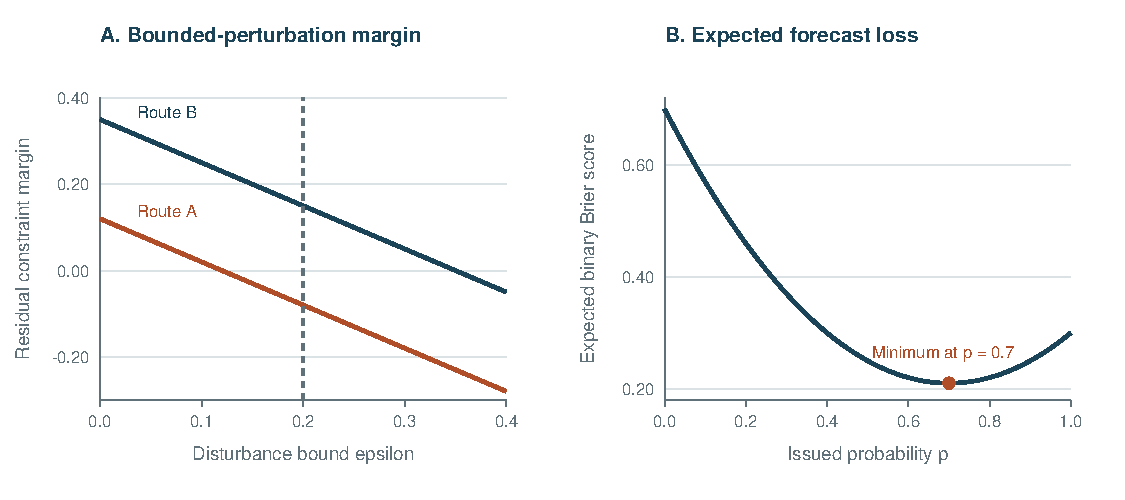
\includegraphics[width=\linewidth]{figures/toy_results.pdf}
\caption{Two deterministic mathematical illustrations. (A) Exact residual margins $c_r-\epsilon$ for abstract corridors; the dashed line marks $\epsilon=0.20$. (B) Expected binary Brier score for a Bernoulli event with $q=0.70$. The plotted curves are calculations, not fitted data.}
\label{fig:toys}
\end{figure}

\subsection{Confidence can increase expected loss}
With true event probability $q=0.70$, forecasts $p=0.50$, $0.70$, and $0.95$ have expected Brier scores $0.2500$, $0.2100$, and $0.2725$, respectively. Moving from a calibrated forecast to an overconfident one increases expected loss despite sounding more decisive. These are expectations under a known toy distribution, not a study showing that a particular training method improves confidence or accuracy.

\subsection{Allocation under uncertain loading}
Three jobs A, B, and C share one nonpreemptive server and are available at time zero. Loading times are independently $S_A\in\{1,5\}$ and $S_C\in\{2,4\}$, each with equal probability; $S_B=2$. Connection deadlines are $(4,3,7)$, delay weights $(1,2,1)$, and miss penalties $(10,8,6)$. For completion time $F_i$, define tardiness $D_i=\max(0,F_i-d_i)$ and a miss when $F_i>d_i$. Finishing exactly at the deadline is not a miss. The server follows a static permutation without idling and without knowing the future loading realizations.

\begin{table}[htbp]\centering\small
\begin{tabular}{lrrr}\toprule
Order & Expected loss & Expected tardiness & Expected misses\\\midrule
BAC & 11.00 & 3.00 & 1.00\\
BCA & 14.00 & 4.00 & 1.00\\
ABC & 18.00 & 4.00 & 1.50\\
ACB & 25.50 & 6.00 & 1.75\\
CBA & 26.00 & 6.00 & 2.00\\
CAB & 27.75 & 7.25 & 1.75\\
\bottomrule\end{tabular}
\caption{Exact enumeration for the four equally likely synthetic loading scenarios. Tardiness is summed across jobs in time units. The loss includes declared priority weights and missed-connection penalties.}\label{tab:schedules}
\end{table}

The best of the six enumerated static orders is \BestOrder{} with expected loss \BestLoss. For BAC the four scenario losses are $0,0,21,23$, whose mean is 11.00. This confirms only optimality within this finite policy class and these four equiprobable scenarios. An adaptive network policy has a different decision space. Changing priorities, deadlines, correlations, or available capacity can change the ranking. No confidential real routes were used, and this calculation supplies no privacy guarantee.

\subsection{The all-or-none bottleneck}
For thirty independent learners with identical success probability, $p^{30}$ is approximately 0.0424 for $p=0.90$, 0.2146 for $p=0.95$, and 0.7397 for $p=0.99$. These values demonstrate sensitivity of a collective endpoint to individual probabilities. They do not estimate any real graduation rate. Peer learning, shared instruction, and group stress can introduce dependence, so both benefit and harm must be evaluated rather than inferred from the formula.

\section{Prospective research protocols}
\label{sec:protocols}
The following are protocol proposals, not registered or completed studies. No sample size, approval, recruitment, clinical benefit, or successful intervention is claimed. Before data collection, freeze hypotheses, randomization, exclusion rules, primary outcomes, analysis code, and a power calculation based on a defensible minimally relevant effect. Simulation should assess the proposed estimator under missingness, realistic clustering, and uncertainty in effect size. A feasibility pilot should inform procedures without being relabeled as a confirmatory trial.

\subsection{Study A: robustness and scheduling benchmarks}
\textbf{Question.} Does a robust policy reduce constraint violations under disturbances represented in its uncertainty set, and at what cost? Compare a nominal optimizer, a robust optimizer, and a simple conservative baseline on released synthetic instances. Vary perturbation magnitude, model misspecification, network congestion, and available information. Freeze scenario generators and test sets separately from algorithm tuning.

\textbf{Outcomes and falsifiers.} Report violation rates with uncertainty, worst observed violation, nominal cost, compute time, missed connections, and unweighted and class-specific delays. An in-set violation despite a valid certificate would expose an implementation error, invalid bound, or violated assumption. Out-of-set failures characterize robustness limits. Report infeasibility explicitly rather than silently dropping difficult instances. Any separate privacy claim requires its own adjacency relation, leakage definition, composition analysis, and proof or adversarial evaluation.

\subsection{Study B: prediction-first physiological calibration}
\textbf{Design.} Randomly assign consenting adults to structured estimate--feedback training or a matched educational control with delayed aggregate feedback. Keep a blinded reference sensor recording in both groups. Predefine posture, estimation windows, rest intervals, display visibility, signal-quality exclusions, and the separate tasks for pulse and respiration. Collect confidence before revealing feedback and record participants' estimation strategies. Include an unfamiliar assessment context and a delayed retention visit.

\textbf{Primary estimand.} The difference between groups in change in held-out heart-rate MAE relative to a specified reference method. Respiration error, signed bias, interval coverage, confidence--accuracy association, and distress are secondary. Use a baseline-adjusted participant-level model or a prespecified hierarchical model; repeated trials are not independent participants. Analyze all randomized participants according to assignment, describe missingness, and perform stated sensitivity analyses. A practically null or adverse effect on the primary outcome would count against the training hypothesis even if self-reported confidence improved.

\textbf{Interpretation.} Performance relative to one device does not establish perfect awareness of internal physiology. Heartbeat counting is not the sole endpoint. The trial would not justify removing medically necessary monitoring or assuming that skill transfers to untested bodily variables.

\subsection{Study C: component testing of embodied updating}
\textbf{Design.} An eight-arm, parallel $2\times2\times2$ factorial study can compare (i) the source-inspired tapping locations versus matched alternative-location touch, (ii) comfortable paced breathing versus a matched period of unpaced breathing, and (iii) an evidence-revision cue versus neutral wording. Session duration, facilitator contact, task instructions, and expected plausibility should be matched as far as possible. Record expectancy and adherence. Participants cannot be fully blinded to action differences; analysts and outcome assessors can be masked to assignment.

\textbf{Task and primary outcome.} Use repeated probabilistic inference tasks with a declared generative model, new evidence, and later binary outcomes. Obtain forecasts before and after evidence, separating any bodily-state change from the factual revision. The primary outcome is mean post-evidence Brier score on held-out tasks, adjusted for baseline performance. Prespecify the main contrast for each factor and adjust for the three confirmatory comparisons; interactions and affective outcomes can be designated secondary unless the study is powered for them. A hierarchical model should account for participant and task dependence.

\textbf{Mechanistic limits.} This design tests tapping-location specificity, breath-pacing contribution, and cue contribution within a matched procedure. It does not isolate every ingredient, establish a meridian mechanism, or directly compare the whole package with no intervention. A separate no-touch control would be needed to estimate the contribution of rhythmic touch itself. Better mood without better inference would support an affective outcome only. More revision when evidence is uninformative could be a harmful increase in suggestibility. Report unchanged and worsening outcomes as well as improvements.

\subsection{Study D: cooperative learning without coercive certification}
\textbf{Design.} Randomize multiple intact learning groups to structured peer support with a collective milestone or to an equally resourced individual-progression program. Preserve individual certification and withdrawal in both arms. This intentionally tests a less coercive implementation of the source's cooperative idea; it is not a literal test of withholding every learner's credential until all pass.

\textbf{Outcomes.} The primary outcome is independently assessed individual mastery on unfamiliar tasks at a fixed follow-up. Secondary outcomes include delayed retention, dispersion of learning gains, time to mastery, helping behavior, assessment integrity, distress, exclusion, and perceived pressure. Assessors should be blind to group assignment. The group is the randomization unit; power and uncertainty must reflect the number of groups and intracluster correlation, not merely the number of learners. A single thirty-person cohort cannot identify the program's causal effect.

\subsection{Consent, data governance, and stopping rules}
Any human study requires prospective review by the responsible ethics body, individual informed consent, a clear withdrawal procedure, and avoidance of academic or interpersonal penalties for declining. Physiological recordings and personal inferences are sensitive data: collect the minimum necessary, separate identities from analysis records, define retention and access, and publish only appropriately governed outputs. The source's paired consent scene does not substitute for these procedures.

Breathing and attention tasks should permit ordinary comfortable breathing, immediate cessation for discomfort, and a prespecified response to adverse events. The proposed study need not use breath holds, hyperventilation, forced disclosure, sleep deprivation, or physical threat. Those would introduce additional interventions and risks unrelated to the central hypotheses. A stopping plan should specify who reviews adverse events and when recruitment or a procedure is suspended. These are research-design requirements, not claims that the narrative's practice is safe or unsafe in every setting.

\clearpage
\section{Connections to the versioned ZoraASI research program}
\label{sec:zora}
\subsection{A shared method does not identify a shared mechanism}
The strongest connection is methodological: distinguish the world from a record of the world, retain uncertainty, make predictions before feedback, and demand that claimed mechanisms survive controls. In ZoraASI these rules become software interfaces, provenance records, abstention policies, and causal memory updates. In the physical research they become defined operators, state preparation, identifiable parameters, controlled approximations, and experimental likelihoods. The similarity justifies transferring evaluation methods; it does not identify neural, computational, and quantum variables with one another.

This expansion uses four connection labels in addition to the original claim classes: \textbf{direct method} for an operational transfer; \textbf{conditional model} for consequences of stated mathematics; \textbf{proposed test} for an unexecuted evaluation; and \textbf{speculative bridge} for a connection without an adequate empirical or mathematical map. ``ZoraASI'' names the research program, not a measured achievement of artificial superintelligence. ``Theory of Everything'' identifies the author's research corpus, not a demonstrated unification.

\begin{table}[htbp]
\centering\small
\begin{tabular}{@{}>{\raggedright\arraybackslash}p{.22\linewidth}>{\raggedright\arraybackslash}p{.37\linewidth}>{\raggedright\arraybackslash}p{.34\linewidth}@{}}
\toprule
Narrative principles & Operational research connection & Evidential boundary\\\midrule
P01--04, P11, P16--18 & Source ancestry, timestamps, preserved evidence, and typed relations in evidence review & Direct method; hashes identify bytes, not truth.\\
P08, P12, P21, P39, P49 & Selective risk, justified abstention, and blinded challenge & Proposed engineering tests; repeated calls can share errors.\\
P10, P24--28, P36, P44, P74 & Prequential scoring, adaptive forgetting, and worst-regime loss & Direct method; simulation benefits depend on the regime.\\
P10, P22, P28, P46--49 & Define physical observables and identifiable parameter combinations & Direct method; a sensor or model output needs a measurement map.\\
P23--27, P36 & Approximation domains, kinetic positivity, and coupled-vacuum stability & Conditional model tests; subsystem consistency is insufficient.\\
P45, P58, P60, P62, P91--92 & Embodiment, intuition, synchrony, and fictional origins & Speculative bridge to physical consciousness; no field measurement supplied.\\\bottomrule
\end{tabular}
\caption{Crosswalk to the research program. Principle identifiers refer to the unchanged narrative catalogue, not to newly established laws.}
\end{table}

\subsection{Evidence review: what the completed pilot actually shows}
The current local evidence-review package contains a completed frozen comparison of four arms, each applied to twelve claims from four source records \cite{pilot}. The older progress description that the comparison was incomplete is superseded by the saved result, completed on October 23, 2026. The version 2 audit inspected the result and its bound hashes without rerunning the model. The new version 3 challenge is reported separately in Section~\ref{sec:local-tests}. Table~\ref{tab:pilot} reports the saved outcomes.

\begin{table}[htbp]
\centering\small
\begin{tabular}{@{}lrrrr@{}}
\toprule
Measure & Original 1 & Original 3 & Revised 1 & Revised 3\\\midrule
Provisional-label matches & 5/12 & 4/12 & 12/12 & 11/12\\
Unnecessary abstentions & 7 & 8 & 0 & 0\\
Incorrect definite judgments & 0 & 0 & 0 & 0\\
Processing errors & 0 & 0 & 0 & 1\\
Decisive coverage & .0833 & .0000 & .6667 & .6667\\
Input plus output tokens & 13,090 & 40,588 & 14,776 & 46,948\\\bottomrule
\end{tabular}
\caption{Saved pilot outcomes. ``1'' means a single pass; ``3'' means three roles using the same model. Correct abstentions can match labels without contributing to decisive coverage. Labels are provisional.}
\label{tab:pilot}
\end{table}

The revised rules distinguish what a source reports from whether its report establishes a broader or current proposition. The relation vocabulary \texttt{entailed}, \texttt{contradicted}, and \texttt{not\_determined} maps to judgments explicitly. The challenger is isolated from the verifier's verdict. These are concrete implementations of P04, P17, P18, and P21. Nevertheless, the pilot gives no accuracy advantage to three roles; the revised three-role arm incurred one incomplete generation. Its extra calls also consumed more tokens. The revision changed multiple features together, so the observed improvement cannot be assigned to the schema alone.

The twelve claims are correlated within four records and use author/programmatically prepared labels awaiting independent review. Zero observed incorrect definite judgments is therefore not a reliable population error bound. No confidence probabilities were collected, so the results are not a calibration measurement. They motivate a held-out study rather than general superiority claims.

For a future system with decision indicator $D_i$ and error indicator $W_i$ on independently adjudicated cases, define
\begin{equation}
 C=\frac{1}{n}\sum_i D_i,\qquad
 R_{\rm sel}=\frac{\sum_i D_iW_i}{\sum_iD_i}.
\end{equation}
Selective risk is undefined when the denominator is zero; zero coverage must not be scored as zero error. Coverage and risk should be evaluated together, with processing failures separately reported and included as failures in an overall endpoint. Selective classification provides an established risk--coverage framework \cite{geifman}; guarantees from a particular classifier and dataset do not automatically transfer to generated evidence judgments.

\subsection{Adaptive memory: observed benefits and counterexamples}
The Phase 2.9 package contains saved per-seed outcomes for 2,200 simulated paths: eleven scenarios, one hundred seeds, and two seed banks \cite{memory29}. Its causal ordering is directly relevant to P16 and P28: predict first, observe the outcome, score that forecast, then update. The shadow base and archived snapshots are shared for weighting comparisons. The saved package records identity checks and an earlier successful test run. In the version 2 audit the thirty-two manifest entries were verified; paired summary statistics were also recomputed from saved seed outcomes. No forecasting run was performed for that audit; Section~\ref{sec:local-tests} now adds fresh forecasts on disjoint seeds.

Let $\ell_{s,j}^{A}$ be the mean Brier loss of policy $A$ in scenario $s$, seed $j$. The paired effect is
\begin{equation}
 \widehat\Delta_s=\frac{1}{J}\sum_{j=1}^{J}
 (\ell_{s,j}^{A}-\ell_{s,j}^{\rm no\ memory}).
\end{equation}
Negative values favor the policy. For fixed-share forgetting with row-gap handling, the \texttt{mixed\_9} primary-bank effect is $-0.0031993$ with pointwise normal 95\% Monte Carlo interval $[-0.0037538,-0.0026448]$; the second bank gives $-0.0032860$. In \texttt{short\_dwell}, the same contrast is harmful: $+0.0018665$ with interval $[0.0016324,0.0021005]$, and $+0.0016869$ in the second bank. These are exploratory intervals without multiplicity correction, conditional on the synthetic generator and seed design. They are not confidence intervals for real-world intelligence or consciousness.

The useful prediction is therefore conditional adaptation: a causal policy might improve the average tradeoff across recurrence and rapid change while controlling worst-regime harm. Universal benefit is already contradicted by the saved fixture. A fair comparator is the best fixed policy selected on the same validation mixture, not an arbitrarily weak default. Weight adaptation and memory replacement must be ablated separately, because replacement changes the archive itself.

The inspected Phase 2.10 directory contains only an adaptive-memory implementation \cite{memory210}. Its referenced base-suite dependency, protocol, tests, and results are absent from that directory. As supplied, it is an incomplete code proposal. The version 3 tests supply the exact existing base-suite dependency in an isolated copy, add causal-invariant checks, and execute a new bounded evaluation; the original directory remains unchanged. Variable names such as valence and continuity describe internal program quantities; they do not establish subjective experience.

\subsection{A prospective, source-level evaluation design}
For evidence review, divide underlying records and time periods before deriving claims. Fit thresholds and prompts on development records only. Independent adjudicators should label both the truth conditions and the scope supported by the supplied evidence, with disagreements retained. Blind the adjudicators to system arm. Repeat identical cases across randomized arm orders and cluster uncertainty by source record, since paraphrases and claims from one record share evidence.

For memory, freeze validation and test generators, seed banks, scenario weights, archive capacity, and compute budgets before inspecting test outcomes. Score each forecast before state updates. Report an equally weighted scenario-average effect and the worst scenario; a favorable aggregate does not erase short-dwell failure. Compare no memory, selected fixed forgetting, a uniform mixture, the adaptive mixture, and TTL under common paths. Repeated seed banks test simulation stability, not transport to a new application.

These designs instantiate the narrative's estimate--measure--revise discipline without borrowing its fictional physiology. They also make a stronger claim falsifiable: engineering improvements should survive matched resources, independent source cases, and adversarially selected failure regimes.

\clearpage
\section{Conditional physics: observables before interpretation}
\label{sec:physics}
\subsection{Three branches that require separate assumptions}
The inspected Theory of Everything records do not specify one empirically completed model. The dated 6,433-page corpus audit identifies a controlled front packet and a Part 0 scalar-modulated open-system effective theory, followed by substantial historical and exploratory material \cite{toeaudit}. A later quadratic Higgs-portal note supplies a microscopic conditional decoherence calculation \cite{portal}. The October 22 scalar/anomaly and exact-mode packages study a specified spectral action \cite{scalar,exact}. Historical Born-bias formulas, classical rate modulation, a quadratic quantum bath, and a compactification calculation must not be combined by identifying symbols that happen to have similar names.

For clarity, write the classical modulator as $\mathcal E$, the bath field as $\varphi$, the Higgs field as $H$, and the spectral scalar amplitudes as $h_i$. A map among these objects would need a common action, symmetry assignments, dimensions, state, normalization, and matching calculation. No such full map is established in the inspected records. The connection to Quiet Calculus P10 and P22 is precisely to preserve that boundary.

\subsection{Classical rate modulation and an information-null test}
The rate branch posits a local classical response
\begin{equation}
 \gamma_k(x)=\gamma_{k0}\exp[\eta_k\mathcal E(x)],\qquad
 (\Box+m_{\mathcal E}^{2})\mathcal E=J.
 \label{eq:rate}
\end{equation}
Here $\eta_k\mathcal E$ is dimensionless and $J$ must be a physically defined source with units and a transfer function. A hidden-sector choice $J=\kappa_{\mathcal E}S^2$ appears as a working model, not a measured source. Positive continuous composition $F(a+b)=F(a)F(b)$ with $F(0)=1$ implies $F(a)=e^{\eta a}$ by applying the continuous additive functional equation to $\log F$. This conditional derivation does not establish why physical sources should compose that way.

The usual completely positive Markovian generator provides a framework for rates and specified channel operators \cite{lindblad}. Local factorization and retarded classical controls can support the sufficient no-signaling result in the dated research packet. They do not supply a unique relativistic completion or make arbitrary state-dependent nonlinear evolution acceptable.

\begin{proposition}[No information in discarded-time population bits]
\label{prop:bits}
Suppose independent identically prepared two-path probes undergo only pure dephasing in the measured path basis, with equal initial path populations. If an observation retains exactly $N$ path-basis bits and discards all timing, every bit string has probability $2^{-N}$ independent of the dephasing parameter $\lambda$. Its classical Fisher information about $\lambda$ is zero.
\end{proposition}
\begin{proof}
With $Z=\operatorname{diag}(1,-1)$, choose the convention
\begin{equation}
 \dot\rho=\frac{\lambda}{2}(Z\rho Z-\rho).
\end{equation}
Then $\dot\rho_{00}=\dot\rho_{11}=0$ and $\rho_{01}(t)=e^{-\lambda t}\rho_{01}(0)$. Each path-basis outcome remains Bernoulli$(1/2)$, and independence gives $P_\lambda(\boldsymbol x)=2^{-N}$. Consequently $\partial_\lambda\log P_\lambda(\boldsymbol x)=0$, and its squared expectation is zero.
\end{proof}

The proposition does not claim that every measurement basis is insensitive. Recombination converts coherence to an output probability. In an ideal interferometer with known phase $\theta$,
\begin{equation}
 p_+(\lambda)=\frac{1+V\cos\theta}{2},\qquad
 V=e^{-\lambda\tau},\qquad
 \mathcal I_1(\lambda)=
 \frac{\tau^2V^2\cos^2\theta}{1-V^2\cos^2\theta}.
 \label{eq:fisher}
\end{equation}
This expression assumes $0<p_+<1$ and known ideal baseline visibility. It is nonzero away from insensitive phases. In a real experiment, uncertain reference contrast, phase drift, and detection efficiencies are nuisance parameters that reduce identifiable information. Likewise, counts in a fixed duration could inform a \emph{separately specified} event rate; pure dephasing alone does not imply that event-count model.

The dated GATE-04 packet accordingly retires a fixed-count QRNG Born-bias endpoint for the rate-only branch \cite{gate04}. A biased count cannot uniquely support that branch, and an unbiased count does not constrain its rate. This is an explicit negative prediction and a useful design exclusion, not a failure to find an exotic signal. Five apparatus objects remain unspecified in that packet: source calibration, source-to-observable transfer, channel operators, nuisance likelihood, and an accessible effect/power interval.

\subsection{Quadratic portal: a conditional, dimensionally explicit bridge}
Use natural units $\hbar=c=k_B=1$. In the symmetric scalar portal convention
\begin{equation}
 V\supset\frac{\kappa_p}{2}\varphi^2H^\dagger H,
 \qquad H=\frac{1}{\sqrt2}\binom{0}{v+h},
\end{equation}
tree-level low-momentum Higgs exchange produces
\begin{equation}
 \mathcal L_{\rm eff}=c_f\varphi^2\bar f f,
 \qquad c_f=\frac{\kappa_pm_f}{2m_h^2},
 \qquad c_N=\frac{\kappa_pf_Nm_N}{2m_h^2}.
 \label{eq:portal}
\end{equation}
Here $f_N$ is the specified nucleon scalar form factor, and $c_N$ has mass dimension $-1$. The scalar-singlet literature supplies a conventional particle-physics context for portal constraints \cite{athron}; its dark-matter abundance and likelihood assumptions must not be imported into a laboratory bath without justification. The local note's symmetric interaction changes the scalar's effective mass in matter. It does not create an additive source from zero field or establish a populated bath.

Assume a free massive homogeneous Gaussian scalar bath at temperature $T$, zero chemical potential, weak coupling, two heavy fixed probe paths separated by $r$, negligible recoil, and the leading Markov limit. The connected zero-frequency noise of the renormalized composite $[\varphi^2]_R$ gives \cite{portal}
\begin{align}
 S(0,r)&=\frac{1}{2\pi^3}\int_m^\infty d\epsilon\,
 (\epsilon^2-m^2)n_\epsilon(1+n_\epsilon)
 \operatorname{sinc}^2\!\left(r\sqrt{\epsilon^2-m^2}\right),\\
 n_\epsilon&=(e^{\epsilon/T}-1)^{-1},\qquad
 \gamma(r)=c_N^2[S(0,0)-S(0,r)],\qquad
 \frac{V}{V_{\rm ref}}\simeq e^{-\gamma(r)\tau}.
 \label{eq:noise}
\end{align}
We use $\operatorname{sinc}u=\sin u/u$, continuously extended at zero. The noise has mass dimension $3$, so $c_N^2S$ is a rate. Ordinary collisional decoherence is an essential competing mechanism, not evidence of this particular portal \cite{hornberger}.

Set $a=m/T$, $b=rT$ and define $K(a,b)=\gamma/(c_N^2T^3)$. Then
\begin{equation}
 K(a,b)=\frac{1}{2\pi^3}\int_a^\infty
 \frac{(x^2-a^2)e^x}{(e^x-1)^2}
 \left[1-\operatorname{sinc}^2\!\left(b\sqrt{x^2-a^2}\right)\right]dx.
 \label{eq:kernel}
\end{equation}
The integrand supplies the exact conditional constraints
\begin{equation}
 K(a,0)=0,\qquad 0\le K(a,b)\le K_\infty(a),\qquad
 K_\infty(a)=\frac{-a\ln(1-e^{-a})+\operatorname{Li}_2(e^{-a})}{\pi^3}.
\end{equation}
For fixed $a>0$, small separation gives
\begin{equation}
 K(a,b)=\frac{b^2}{6\pi^3}\int_a^\infty
 (x^2-a^2)^2\frac{e^x}{(e^x-1)^2}\,dx+O(b^4).
\end{equation}
Thus $\gamma(2r)/\gamma(r)\to4$ as $rT\to0$ at fixed state. At large separation the rate approaches $c_N^2T^3K_\infty$, and for $m/T\gg1$,
\begin{equation}
 \gamma(\infty)\simeq\frac{c_N^2}{\pi^3}(mT^2+T^3)e^{-m/T}.
\end{equation}
The massive-bath zero-frequency rate vanishes as $T\to0$ under these assumptions; finite switching transients are outside that assertion. A general monotonicity claim is unnecessary because the sinc kernel oscillates. Equal mean fields on two paths also do not imply zero difference noise.

\begin{figure}[htbp]
\centering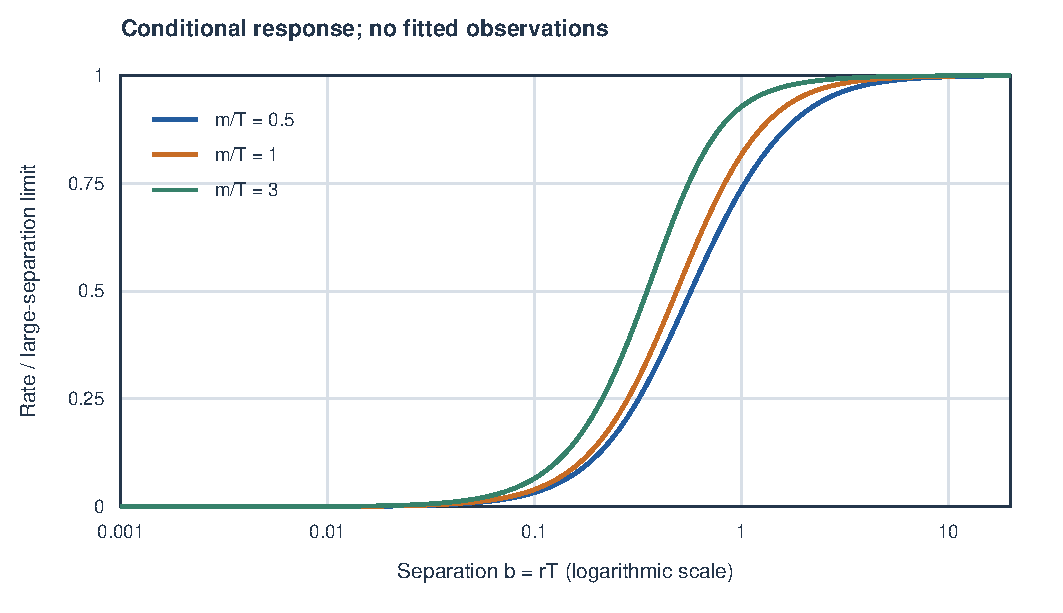
\includegraphics[width=.96\linewidth]{figures/portal_shape.pdf}
\caption{New deterministic illustration of Eq.~\eqref{eq:kernel}: normalized separation response at prescribed $m/T$. Curves are conditional calculations with no fitted data or laboratory amplitude. The small-separation slope is quadratic and the large-separation limit is one. The accompanying JSON records quadrature convergence checks.}
\label{fig:portal}
\end{figure}

For the same prepared bath and probe, ratios of nonzero rates at two separations cancel $c_N^2$. The ratio is undefined at zero coupling or zero reference rate, and its measurement becomes ill-conditioned near that limit. Composite probes require form factors and full path histories; the point-nucleon curve cannot simply be multiplied by a mass-squared factor for an arbitrary apparatus.

\subsection{Cross-channel matching and identifiability limits}
If $m<m_h/2$, the same convention gives
\begin{equation}
 \Gamma_{h\to\varphi\varphi}=\frac{\kappa_p^2v^2}{32\pi m_h}\beta,
 \qquad \beta=\sqrt{1-4m^2/m_h^2}.
\end{equation}
Eliminating $\kappa_p^2$ yields the conditional cross-channel relation
\begin{equation}
 \gamma_N(r)=\frac{8\pi f_N^2m_N^2}{v^2m_h^3\beta}
 \Gamma_{h\to\varphi\varphi}\,[S(0,0)-S(0,r)].
 \label{eq:cross}
\end{equation}
An invisible-width constraint applies only if the daughter particles are invisible in the relevant analysis and its production/width assumptions are satisfied. This paper inserts no numerical collider limit and performs no joint fit. The bath population remains an independent physical input: an upper bound on the coupling does not impose a positive lower bound on laboratory decoherence.

Identifiability is the central difficulty. In Eq.~\eqref{eq:rate}, the transformation $\mathcal E\mapsto A\mathcal E$, $\eta\mapsto\eta/A$ leaves the rate unchanged unless the source scale is independently calibrated. In Eq.~\eqref{eq:noise}, unknown occupation can trade against coupling strength. Shape measurements can constrain some combinations but do not recover all microscopic parameters. A shared fitted damping curve is compatible with several ordinary environmental models. A discriminating analysis needs independent state information, variation of separation and duration, conventional background measurements, and a frozen nuisance likelihood.

\subsection{Exact spectral calculations: approximation control and symmetry}
The scalar/anomaly and exact-mode packages define a separate parity-even classical spectral action \cite{scalar,exact},
\begin{equation}
 S_{\rm sp}=\frac{\kappa_s}{2}\operatorname{Tr}_{\rm Dirac}
 f(D_6^2/\Lambda^2),\qquad
 f(z)=\sum_a w_ae^{-az},\quad a,w_a>0,\quad\sum_aw_a=1.
\end{equation}
The stated geometry is a round internal sphere with $R=\Lambda r$, prescribed monopole sectors and four copied repaired Weyl blocks. Opposite six-dimensional chiralities are inherited assumptions. The geometric weak lift retains its Pauli/curvature vertex. The scalar convention uses $\Phi_i=r^{-1}H_iY_{1/2}$ and $h_i=H_i/(\Lambda R)$; bare amplitudes $h_i$ are not canonical physical vacuum expectation values.

Two admissible profiles share six retained local quantities but differ in exact finite-radius response. At the prescribed $R_*=1.2784724120\ldots$, four blocks, unit dimensionless Yukawas, and profile $f_-$, the saved exact coefficients are
\begin{align}
 C_0&=1.3093131218\times10^{-4},&
 C_1&=2.0841549984\times10^{-4},\\
 C_0+C_1&=2A_4,& C_1/C_0&=1.5917926458\ldots .
\end{align}
The local $a_2$--$a_4$ approximation instead gives $C_0=C_1=1.9351057742\times10^{-4}$. A parallel-flavour identity protects their sum, not their equality. The exact low-momentum quadratic parameter $2A_2/G=-1.7615373631\ldots$ differs from the local $-1.4901575034\ldots$ by about 18.21\% in magnitude. It is not a computed pole mass. These results make P10 and P22 concrete: preserving selected summaries does not identify the full response.

For neutral aligned backgrounds the stipulated charge $Q=J_3+q_Y$ commutes with the background operator. Consequently the neutral mass matrix satisfies
\begin{equation}
 M^2N=0,\qquad N=(1,1,0)^T,\qquad e^{-2}=N^TKN,
\end{equation}
where $K$ is the neutral kinetic matrix and the other directions are assumed massive. A pure-$X$ St\"uckelberg term preserves that direction. At the fixed $f_-$ fixture,
\begin{equation}
 \frac{e^{-2}}{\kappa_s}=0.3999904283
 -0.03932044965h_d^2-0.03773847661h_u^2+O(h^4).
\end{equation}
The difference between the unbroken profiles is $1.5519080\times10^{-7}$, or approximately $3.87986\times10^{-7}$ relatively. This compares mathematical profiles at a fixed bare fixture; it is not a predicted temporal variation of the measured fine-structure constant. The exact continuation also corrects the predecessor's weak-kinetic claim: its geometric $WW$ Higgs correction already has an $a_4$ curvature contribution, rather than first appearing at $a_6$.

The exact bundle records 126 passing checks and its twenty-two manifest entries match. Those are saved computational checks and current file-integrity findings, not 126 experiments. A consistency identity preserved by many theories cannot uniquely confirm this spectral construction.

\subsection{A coupled-vacuum gate and a candidate running observable}
The earlier local scalar fixture found no flat stationary radius within its sampled interval $0.1\le R\le30$ or its stated asymptotic analysis, but its scalar minimum also violated its expansion domain. The exact continuation evaluates fixed-radius coefficients and does not solve a replacement coupled vacuum. Therefore neither record supplies a physical vacuum for the entire proposed completion.

A valid gate must solve joint stationarity and flatness in a declared truncation, remove gauge directions, require positive physical kinetic eigenvalues, and test the kinetic-normalized Hessian for unwanted instabilities. It must also calculate the six-dimensional anomaly polynomial and actual two-form reduction: cancellation among four-dimensional zero modes does not prove higher-dimensional consistency. Failure rejects the specified completion, not every possible theory using similar vocabulary. A bounded numerical search must remain labeled bounded unless supplemented by analytic or interval guarantees.

The saved charge bookkeeping gives the one-loop coefficients
\begin{equation}
 (b_3,b_2,b_Y,b_X,b_{YX})=
 \left(-\frac{17}{3},-\frac53,\frac{83}{9},\frac{316}{3},0\right).
\end{equation}
Under exactly that active matter content, charge convention, and a threshold-free perturbative energy interval,
\begin{equation}
 \frac{d g_i^{-2}}{d\ln\mu}=-\frac{b_i}{8\pi^2},\qquad
 \frac{d(g_Y^{-2}-g_2^{-2})}{d\ln\mu}=-\frac{49}{36\pi^2}.
 \label{eq:running}
\end{equation}
The difference removes a constant matching offset. It does not remove dependence on particle content, thresholds, higher orders, or measured scattering inputs. Four chiral generations in the stipulated notes require an explicit phenomenology audit before this can be presented as a viable model of observed matter. No such viability conclusion is established here. Similarly, $b_{YX}=0$ for complete active multiplets does not eliminate finite mixing from unequal thresholds.

The tree-level massless CP-odd physical scalar in the stipulated two-doublet-plus-axion construction is another conditional symmetry result. QCD effects and allowed operators can lift it; an independently predicted physical mass and coupling are absent. It is a future matching problem, not a claimed detectable axion signal.

\clearpage
\section{Twelve discriminating predictions and research gates}
\label{sec:predictions}
\subsection{Readiness, endpoints, and interpretation}
The following cards were introduced as unexecuted proposals in version 2. They remain the target definitions; version 3 executes feasible subsets in Section~\ref{sec:local-tests}, with exact coverage and remaining gaps reported there. Version 4 adds the targeted revision evaluations in Section~\ref{sec:revisions}; it preserves the original target definitions and historical outcomes. They are not public registrations or claims that every hypothesis will succeed. Z1--Z4 are engineering hypotheses; F1 is an exact negative consequence of a stipulated model; F2--F4 are conditional physical targets; T1--T2 are computational predictions; T3 is a consistency gate with no assumed successful outcome; T4 is a candidate empirical target requiring further matching. Their common form is an explicit observation, a comparator, and a result that would count against the claim.

Version 2 prioritized Z1, a prospective memory test after completing the isolated Z3 package, and an independent numerical T1 route. Version 3 now executes the bounded Z3 comparison and selected T1 routes; the full Z1 factorial and broader independent replication remain open. The most discriminating laboratory candidates are the joint separation--duration--state dependence in F2 and the shared-parameter relation in F3, but both remain conditional on an operational apparatus and independently constrained bath. A bare damping signal would be weak evidence because ordinary decoherence also damps visibility. T3 should precede claims that the spectral branch describes a physical vacuum; T4 requires a credible spectrum and threshold map first.

Each superiority claim should specify a scientifically meaningful effect $\delta$ before data collection and report its interval. For a paired loss difference $\Delta$ where smaller is better, a possible decision rule is an upper confidence bound below $-\delta$. A separate noninferiority guardrail requires its upper bound below a predeclared harm margin. An interval crossing the margin is inconclusive, not proof of equivalence or mechanism absence. For a one-sided normal approximation, a planning quantity is
\begin{equation}
 n_{\rm independent}\simeq
 \frac{(z_{1-\alpha}+z_{1-\beta})^2\sigma_d^2}{(\Delta_1-\Delta_0)^2},
\end{equation}
where $\Delta_0=-\delta$ is the superiority boundary, $\Delta_1<\Delta_0$ is the assumed true effect, and $\sigma_d^2$ is the independent-cluster paired-difference variance. It is not a numerical sample-size prescription for the four-record pilot. The required variance and meaningful margins need external justification or separate pilot data. Source clusters, multiple endpoints, repeated looks, and selection of the best baseline must enter the final design. Choose one confirmatory primary contrast per study or predeclare familywise control; retain exploratory analyses as exploratory.

\subsection{ZoraASI engineering cards}
\paragraph{Z1: Explicit evidence relations reduce avoidable abstention.}
\textbf{Prediction and endpoint:} the revised scope rules and relation schema reduce unnecessary abstention on answerable unseen claims without exceeding a prespecified increase in incorrect definite judgments. \textbf{Comparison:} frozen original versus revised single-pass systems, followed by a rules-by-schema factorial ablation. \textbf{Controls:} identical evidence and model digest, held-out records and dates, independent scope/truth labels, blinded adjudication, clustered inference, and failures included in an overall endpoint. \textbf{Decision:} support requires the abstention reduction and the false-certainty guardrail together. A coverage increase alone fails the claim. The existing twelve-case result selects a candidate; it does not estimate a transportable effect. \textbf{Readiness:} protocol specification and independent labels required; no novel physics required.

\paragraph{Z2: Blinded challenge helps through error diversity.}
\textbf{Prediction and endpoint:} hiding the verifier's verdict from the challenger lowers selective error at a prespecified common coverage. \textbf{Comparison:} blind versus informed challenger within the same three-role architecture, plus a single-pass baseline matched on actual resource budget. \textbf{Controls:} identical source families, randomized arm order, separate measurements of joint verifier/challenger mistakes, truncation, tokens, and latency. \textbf{Decision:} no error reduction at matched coverage/cost, or a benefit explained entirely by refusing more cases, fails the proposed advantage. Equal total output allowance does not by itself equalize repeated input cost or truncation risk. \textbf{Readiness:} engineering experiment; the saved pilot currently gives no three-role accuracy gain.

\paragraph{Z3: Adaptive forgetting improves the recurrence--change tradeoff.}
\textbf{Prediction and endpoint:} a causal mixture of forgetting rates improves equally weighted held-out scenario-average Brier loss relative to the best fixed rate selected on the same validation mixture, subject to worst-scenario and stationary-regime harm limits. \textbf{Comparison:} selected fixed rate, adaptive mixture, uniform mixture, no memory, and TTL. \textbf{Controls:} common paths, disjoint seeds, prequential scoring, identical shadow base/archive for weighting ablations, and separate replacement-policy factors. \textbf{Decision:} lack of improvement over the strongest selected baseline or violation of the guardrail fails the bounded claim. Phase 2.9's short-dwell counterexample rules out unconditional benefit. \textbf{Readiness:} the original Phase 2.10 bundle lacks a dependency and a complete test package. The isolated version 3 experiment supplies these locally and evaluates a specific frozen comparison; broader robustness remains open.

\paragraph{Z4: Provenance awareness resists duplicated and stale evidence.}
\textbf{Prediction and endpoint:} source-ancestry and time metadata reduce increases in false definite judgments under duplication or obsolete-report perturbations while preserving appropriate use of genuinely new evidence. \textbf{Comparison:} metadata present versus ablated with paired, truth-preserving perturbations: duplicates, independent corroboration, superseded reports, unavailable current records, and authentic but irrelevant quotations. \textbf{Controls:} equalized context/source budgets, blinded semantic labels, fixed underlying propositions, and record-level clustering. \textbf{Decision:} unwarranted certainty rises materially under duplicate/stale evidence, or independent corroboration cannot be distinguished from copying. Numerical confidence scoring is a new endpoint if added; it cannot be inferred from the existing verdict labels. \textbf{Readiness:} controlled evidence benchmark.

\subsection{Conditional physical cards}
\paragraph{F1: Fixed-count population bits are insensitive to pure dephasing.}
\textbf{Prediction:} under Proposition~\ref{prop:bits}, bit-value distributions and their likelihood have zero dependence on the dephasing rate. \textbf{Comparison:} retain path-basis bits versus recombined, phase-resolved interference data from the same stipulated dynamics. \textbf{Observable:} likelihood derivative or estimated rate information, not a post hoc bit imbalance. \textbf{Controls:} known preparation, readout basis, independence, fixed count, and timing exclusion; the interference model must retain nuisance contrast and phase. \textbf{Failure interpretation:} parameter dependence in the exact stipulated bit model rejects the implementation or an assumption. A laboratory bias suggests preparation, readout, population transfer, or another mechanism; it is not distinctive support for rate-only physics. \textbf{Readiness:} analytic and software test available now; it does not require a claimed field detection.

\paragraph{F2: Quadratic-portal decoherence has a constrained spatial shape.}
\textbf{Prediction:} the massive thermal weak-coupling point-probe model gives zero rate at coincident paths, quadratic small-separation scaling, a finite saturation value, and the stated low-temperature activation. \textbf{Observable:} $-\log(V/V_{\rm ref})/\tau$ over several separations, durations, and independently characterized bath states; a ratio at two nonzero rates removes the shared coupling. \textbf{Comparison:} the full kernel versus conventional noise mechanisms and a generic fitted damping curve, with identical nuisance treatment. \textbf{Decision:} a jointly incompatible shape rejects the frozen bath/portal/apparatus model after quantified systematics. Agreement does not uniquely identify a scalar. No signal cannot reject arbitrarily weak coupling or absent bath population. \textbf{Readiness:} conditional numerical curve supplied here; finite trajectories, composite form factors, bath preparation, and power remain open.

\paragraph{F3: One portal parameter must fit both width and visibility.}
\textbf{Prediction:} Eq.~\eqref{eq:cross} holds when the same scalar, normalization, mass, and portal account for Higgs decay and the prepared probe environment. \textbf{Observable:} a joint likelihood for the width and visibility kernel with independently constrained bath occupation and nuclear inputs. \textbf{Comparison:} a single shared coupling versus unrelated effective amplitudes, including ordinary decoherence. \textbf{Decision:} no allowed shared parameter region rejects the specified common explanation, conditional on nuisance and model adequacy. A width upper limit by itself supplies no lower bound on visibility loss. \textbf{Controls:} invisibility assumptions, thresholds, data overlap, total-width conventions, and absence of double counting. \textbf{Readiness:} algebraic bridge available; no joint empirical fit or new exclusion is reported.

\paragraph{F4: Calibrated rate modulation obeys a composition constraint.}
\textbf{Prediction:} if two calibrated source contributions add in $\mathcal E$, the exponential response satisfies
\begin{equation}
 \log\!\left[\frac{\gamma(\mathcal E_1+\mathcal E_2)\gamma(0)}
 {\gamma(\mathcal E_1)\gamma(\mathcal E_2)}\right]=0.
\end{equation}
\textbf{Observable:} a source-factorial rate contrast with positive rates and fixed channel/readout. \textbf{Comparison:} exponential, linear-response, saturating, and ordinary environmental models over a predeclared range. \textbf{Decision:} a contrast incompatible with zero rejects additive exponential response under the calibrated source assumptions. Small-signal agreement is weak discrimination because many models share a linear Taylor term. \textbf{Controls:} independent field/source calibration, baseline drift, nonlinear source transfer, nuisance rates, and held-out amplitude levels. \textbf{Readiness:} source and apparatus objects remain open; cognitive or ethical labels are not calibrated physical sources.

\subsection{Spectral and consistency cards}
\paragraph{T1: Exact finite-radius kernels split the local mixed quartics.}
\textbf{Prediction:} for the fixed supplied operator, profile, radius, and scalar convention, $C_0+C_1=2A_4$ while $C_1/C_0\simeq1.59179265$, not one. \textbf{Comparison:} independent block-exponential and Cauchy-contour implementations, increased angular cutoffs, and the local approximation. \textbf{Observable:} coefficient differences and cutoff convergence. \textbf{Proposed tolerances:} absolute coefficient agreement $10^{-9}$ and sum-identity residual $10^{-10}$, to be frozen alongside precision and cutoff rules. These tolerances are new protocol choices, not observed errors. \textbf{Decision:} persistent disagreement after controlled convergence rejects the stated calculation; recovery of unequal coefficients does not reject it. \textbf{Readiness:} independent computational replication can proceed from the saved package. Physical masses require further normalization and vacuum matching.

\paragraph{T2: The protected photon direction survives the scalar response.}
\textbf{Prediction:} neutral alignment and the stipulated charge imply $M^2N=0$, while the kinetic residue follows the quoted quadratic response. \textbf{Comparison:} an independent full external-Clifford finite-momentum implementation versus the saved reduction. \textbf{Observable:} a scale-normalized mass-null residual, the scalar--gauge Ward relation, and a remainder scaling as $O(h^4)$ after subtracting the quadratic term under uniform field rescaling. \textbf{Decision:} a residual surviving precision/cutoff control or a remainder inconsistent with the $O(h^4)$ bound rejects the specified calculation. Roundoff near zero must be controlled. \textbf{Readiness:} computational test; photon masslessness is common to other gauge theories and is not distinctive empirical confirmation of this construction.

\paragraph{T3: A complete benchmark must pass coupled consistency.}
\textbf{Gate, not an assumed positive prediction:} in one frozen scheme solve joint radius/scalar stationarity and flatness, require positive physical kinetic eigenvalues and an acceptable normalized Hessian after removing gauge directions, then compute and cancel the appropriate higher-dimensional anomalies with stipulated fields/counterterms. \textbf{Comparison:} exact treatment versus controlled truncations inside their own domains. \textbf{Decision:} no admissible solution in a rigorously covered domain, a forbidden physical instability, or an uncancelled irreducible anomaly rejects that benchmark. An unsuccessful bounded numerical search is only a bounded search result. \textbf{Controls:} fixed allowed parameters and counterterms; no unregistered rescue term. \textbf{Readiness:} unresolved theoretical work. Success would establish conditional consistency, not observed unification.

\paragraph{T4: A fixed light spectrum predicts relative running slopes.}
\textbf{Prediction:} in a predeclared threshold-free interval with the stipulated active matter, Eq.~\eqref{eq:running} fixes the relative inverse-coupling slope. \textbf{Observable:} multi-scale scattering observables translated using a single matching scheme and covariance model. \textbf{Comparison:} the frozen joint slope vector versus alternatives with different independently specified spectra; constant matching offsets may float. \textbf{Decision:} incompatible slopes reject that spectrum/completion at the declared perturbative accuracy. Choosing thresholds from the same test data destroys the claimed out-of-sample prediction. \textbf{Controls:} physical masses, hypercharge normalization, thresholds, higher-order errors, and correlated datasets. \textbf{Readiness:} phenomenology and spectrum audit required, especially for the four chiral generations. No measured running fit is performed here.

\subsection{Explicit ledger of speculative connections}
\begin{longtable}{@{}>{\raggedright\arraybackslash}p{.25\linewidth}>{\raggedright\arraybackslash}p{.34\linewidth}>{\raggedright\arraybackslash}p{.34\linewidth}@{}}
\toprule
Speculative bridge & What the record supports & What would be needed\\\midrule
\endfirsthead
\toprule Speculative bridge & What the record supports & What would be needed\\\midrule\endhead
\bottomrule\endfoot
Functional self-monitoring implies experience & Forecasts and internal-state variables can be operationally scored. & An independent theory and validated discriminating measurements of experience; performance labels alone are insufficient.\\
Cognitive valence or coherence is $\mathcal E$ or $\varphi$ & Software and physiological quantities have domain-specific definitions. & Units, an observable field estimator, causal source manipulation, coupling action, controls, and replicated data.\\
Ethical intention sources a physical field & Normative constraints can govern choices and experiments. & A noncircular physical source definition and falsifiable controlled effect; a moral score is not a source term.\\
Narrative branch selection is quantum outcome control & The source explicitly uses metaphor/toy descriptions; the inspected rate branch preserves population probabilities. & A different explicit dynamics, consistency checks, and distinctive observations. It cannot be inferred from a fictional scene.\\
Machine memory resembles biological inheritance & Memory policies admit causal software ablations. & A biological mechanism, genotype/phenotype measurements, and independent evidence for any inherited architecture.\\
One unified consciousness--matter theory follows from common mathematics & Several branches use constraints, noise, feedback, and symmetry. & A single action and consistent limits, matched scales/parameters, identified observables, and successful independent tests. Shared vocabulary does not supply that bridge.\\
\end{longtable}

Keeping these entries explicit makes exploration possible without turning an analogy into a result. A speculative bridge can become a conditional model when its variables and equations are defined, and an empirical claim only when a suitable observation is supplied. It need not be deleted from the research agenda; it must retain its current evidential status.

\clearpage
\section{Executed local tests: computational results and limits}
\label{sec:local-tests}
\subsection{Design, preservation, and evidence classes}
Version 3 executes a bounded local campaign against feasible portions of the prediction program \cite{localtests}. Original research directories and synced project sources remain unchanged. Each workstream uses an isolated copy, records runtime versions and commands, and hashes its protocol and executable files before the new executions. Historical results and the scenario families were already known. These freezes prevent silent revision of the recorded plan; they are not independent, blinded, public preregistration. A numerical diagnostic added after observing integration warnings is explicitly exploratory and preserves the first result.

The campaign separates four evidence classes. \emph{Software checks} test code invariants and defined failure behavior. \emph{Synthetic inference evaluations} observe the output of an actual local language model on authored evidence problems. \emph{Simulation experiments} compare prediction algorithms on generated paths with known outcomes. \emph{Mathematical numerical checks} compare implementations and consequences of stipulated equations. The second and third classes provide computational performance evidence within their constructed tasks. None supplies a laboratory observation, a measured new field, a consciousness measurement, or a completed physical Theory of Everything.

Check counts are not counts of independent physical experiments. Several tests share code, generators, states, source builders, or identities. Protocol thresholds are declared engineering/numerical choices, not universal standards. A passed assertion validates only what the assertion actually tests; a failed comparison must be interpreted at the level of its assumptions and numerical reliability.

\subsection{Local inference: shared semantic errors survive three roles}
The isolated revision-3 evidence-review system was evaluated on twelve new, AI-authored fictional event groups, with four provisional supported, four refuted, and four insufficient-evidence labels. Each group contributed one claim. The cases were authored before inference and include absent efficacy evidence, temporally stale reports, copied sources, and unresolved conflict. They share templates and are not a representative independent sample of real-world claims. Labels follow frozen author-specified scope rules and have not received independent human adjudication.

The revised single-pass and blind three-role systems used the same local \texttt{zora:fast} model, with its full digest recorded in the evidence bundle. The final dataset and protocol were sealed before the first inference; one preflight wording correction and its earlier freeze are retained. All twenty-four arm outcomes and forty-eight inference calls completed within the frozen sixty-second per-call and twenty-minute overall limits. There were no retries, processing failures, truncation failures, or post-outcome label/prompt changes. Exact requests and full responses are preserved.

\begin{table}[htbp]
\centering
\begin{tabular}{@{}lrr@{}}
\toprule
Measure & Single pass & Three roles\\\midrule
Matches to provisional labels & $10/12$ & $10/12$\\
Definite-judgment coverage & $10/12$ & $10/12$\\
Errors among definite judgments & $2/10$ & $2/10$\\
Correct abstentions among undecidable claims & $2/4$ & $2/4$\\
False confirmations & 0 & 0\\
Processing failures & 0 & 0\\
Total input and output tokens & 9,682 & 31,769\\
Sum of case wall times (s) & 122.850 & 445.783\\
\bottomrule
\end{tabular}
\caption{Fresh bounded synthetic inference evaluation. Both systems make the same two errors. Equal generation allowance does not equalize total computation. These descriptive rates are not estimates of population accuracy or probability calibration.}
\label{tab:fresh-pilot}
\end{table}

Both arms falsely refuted two undecidable propositions under the frozen rules. In Q03, a recommendation document omitted efficacy results; absence of results in that document was treated as proof that experimental verification did not exist. In Q12, two contemporaneous sources disagreed at the same scope; neither had frozen priority, yet the negative report was selected as a definitive refutation. All four mistaken answers cited genuine source text. Quote membership therefore coexisted with wrong semantic judgments.

Three roles used $3.28$ times the reported tokens and $3.63$ times the wall time without an aggregate improvement on this set. The three-role arm contained one verifier/challenger disagreement. This is neither a superiority nor an equivalence test, and does not isolate the causal effect of blinding: there is no informed-challenger arm or resource-matched baseline. The completed run took approximately 569 seconds. No probabilities were requested, so probability calibration was not measured.

Twenty-nine original regression tests and 668 fresh integrity/control assertions passed. The controls cover future timestamps, tampering, context limits, copied-source dependence, hidden label fields, and relation mapping. One deliberate control supplied a wrong verdict with an authentic quotation: the traceability validator accepted it, exactly as its narrower contract permits. This is a successful demonstration of a limitation, not successful semantic validation. A separate 380-check artifact/arithmetic audit verified raw inputs and outputs, frozen hashes, blind challenger inputs, token accounting, and reported metrics. These are software checks, not additional independent claims or physical experiments.

The observed failure mode is shared semantic overreach despite authentic evidence and multiple roles. Z1's original-versus-revised comparison and Z4's metadata ablation remain unperformed, while the particular causal Z2 blinding hypothesis remains open. The new run gives bounded model-behavior evidence and a concrete challenge for future independent adjudication; it does not establish general ZoraASI capability, consciousness, or physical theory validity.


\subsection{Adaptive memory: small mean gain fails the robustness criterion}
The unchanged Phase 2.10 implementation was made runnable in isolation by supplying the exact existing Phase 2.5 reference dependency. Twenty-three inherited engine tests, nine harness tests, and nine new causal-invariant tests passed: forty-one software checks. These establish bounded implementation properties, not an adaptive-memory benefit by themselves.

The frozen comparison used six candidate fixed hazards, no replacement in the primary weighting arms, a shared base/archive, and an adaptive hazard mixture. Twenty new validation seeds per scenario selected fixed hazard $0.05$ by equally weighted mean Brier loss across eleven unchanged scenario generators. The selection was saved and hashed before test outcomes. Two disjoint test banks of fifty seeds each then generated 1,100 scenario paths. Seeds and their training offsets were disjoint from the known prior banks; the scenario families themselves were familiar.

The primary estimand averages the eleven paired scenario differences within each seed and then over the one hundred seed clusters. The test therefore does not treat time steps or eleven scenarios sharing a seed as independent observations. For adaptive minus selected-fixed Brier loss, the combined mean is
\begin{equation}
 \widehat\Delta=-0.000279697,\qquad
 \text{95\% Monte Carlo interval}=[-0.000334106,-0.000225288].
\end{equation}
The two bank means are $-0.000314317$ and $-0.000245077$, both favoring the adaptive policy. These normal intervals quantify variation under the specified generators and seed design, not uncertainty about general intelligence or application transfer.

The frozen decision required negative means in both banks, a one-sided 95\% upper bound below $-0.0005$ \emph{and} all eleven one-sided Bonferroni-adjusted scenario bounds below a $+0.001$ harm margin. The primary upper bound is $-0.000234036$, so the minimum-effect criterion fails. The worst mean scenario, \texttt{mixed\_9}, has difference $+0.00180538$ and simultaneous upper bound $+0.00189061$, so the robustness guardrail also fails. These margins were bounded engineering choices made before execution, not established utility thresholds.

The heterogeneity is substantial: \texttt{short\_dwell} improves by $-0.00673905$ with pointwise interval $[-0.00698945,-0.00648865]$, while \texttt{mixed\_9} worsens by $+0.00180538$ with interval $[0.00174135,0.00186942]$. Figure~\ref{fig:memory-test} shows all eleven scenarios. This does not reverse the earlier Phase 2.9 comparison: the new contrast uses a different adaptive policy and a validation-selected fixed-memory baseline, whereas the earlier result compared share-gap memory with no memory.

\begin{figure}[htbp]
\centering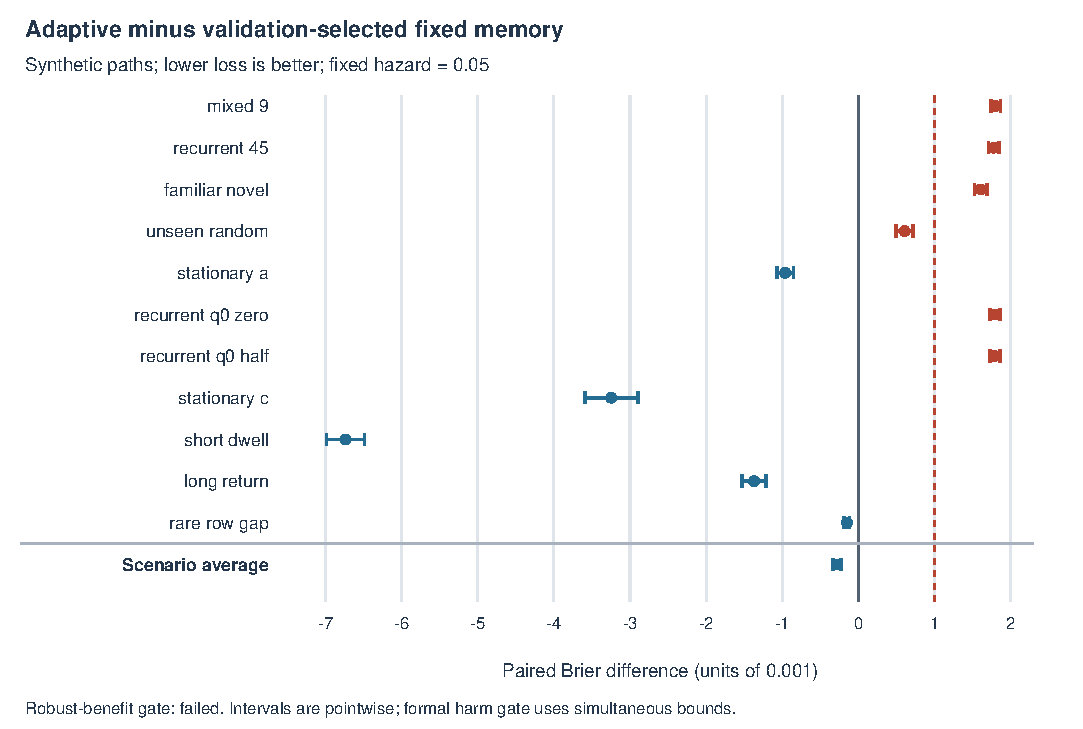
\includegraphics[width=.96\linewidth]{figures/fresh_memory_results.pdf}
\caption{Fresh computational memory evaluation. Points and bars are paired mean Brier differences and pointwise normal 95\% Monte Carlo intervals over one hundred seed clusters. Negative favors adaptive memory. The dashed $+0.001$ line shows the chosen harm margin; the formal guardrail uses separate Bonferroni upper bounds, not these pointwise bars. The overall row is the equally weighted within-seed scenario average. Known synthetic families and fresh seeds do not constitute external application validation.}
\label{fig:memory-test}
\end{figure}

All paths completed without processing or identity-assertion failures. The main adaptive and fixed arms accumulated 41.73 and 15.92 seconds respectively within an approximately 271-second evaluation, including verification overhead; this was not a resource-matched contest. Log loss, uniform mixtures, no-memory, TTL, and replacement-policy contrasts are retained as descriptive secondary results. No prompts or algorithms were tuned after outcomes.

The bounded conclusion is a small mean predictive improvement with important harms, and failure of this particular Z3 robust-benefit criterion. It does not establish equivalence, universal failure of adaptation, or a successful remedy. An amended algorithm would require a new frozen evaluation rather than reclassifying these test paths as fresh validation data.



\subsection{Quadratic portal: an independent reference also needs testing}
The unchanged inherited quadratic-portal checker executed successfully in isolation. Its analytic matching, original twenty-four-case quadrature grid, limiting checks, mixed-scalar checks, covariance fixture, and explicit negative controls passed. The new stress sweep compared the inherited energy-variable quadrature with an adaptive radial collision-flux integral over $m/T\in\{0.01,0.1,0.3,1,3,10,30,100\}$ and $rT\in\{0,10^{-6},10^{-3},0.1,1,10,50\}$: fifty-six cases spanning a wider range than the original grid.

The initial plan did \emph{not} achieve an all-pass result. Forty-seven cases met the reference-convergence and agreement criteria; nine produced adaptive-quadrature warnings. Two raw comparisons exceeded the frozen $10^{-7}$ tolerance relative to the local spectrum, with maximum discrepancy $5.65\times10^{-7}$. Because the candidate reference itself warned, this was a numerical reliability failure, not a justified rejection of the inherited formula or its physical assumptions. All initial warnings and failed flags remain in the package.

A separately frozen exploratory follow-up integrated radial momentum on intervals adapted to the oscillation phase, comparing Gauss orders 16 and 32. All fifty-six inter-order differences were below $10^{-10}$ of the local spectrum; the maximum was $5.31\times10^{-11}$. For the sixteen cases with $rT\ge10$, a distinct weighted-cosine representation gave maximum disagreement $5.45\times10^{-16}$, without warnings. Its use follows from rewriting $\operatorname{sinc}^2(kr)=[1-\cos(2kr)]/(2k^2r^2)$; it resolves an oscillatory residual rather than relying on an adaptive integral of the nearly saturated total rate.

Against the resolved reference, the largest inherited-grid discrepancy was $8.77\times10^{-8}$, and no case exceeded the original $10^{-7}$ agreement threshold. Refining the inherited energy grid in memory, without changing the physical kernel or original file, reduced the maximum discrepancy to $6.13\times10^{-15}$. The largest initial mismatch was traced to the adaptive reference; in the other threshold-exceeding case, both initial quadratures contributed comparably. This is an exploratory numerical diagnosis, not a retroactive all-pass claim for the initial protocol, and the quadrature comparison is not a rigorous error enclosure over all parameters.

Twelve additional twelve-position covariance configurations had positive minimum eigenvalues; the smallest eigenvalue normalized by the local spectrum was $0.2785$. A deliberately quarter-normalized rate disagreed with the independent normalization by $75\%$ and was detected. These tests support internal normalization and positivity on the tested fixtures. They do not establish the existence, population, temperature, or coupling of a physical scalar bath, and do not test an apparatus-specific F2 or F3 signal.

\subsection{Pure dephasing: implementation checks and informative controls}
For F1, direct exponentiation of the $4\times4$ Liouvillian was compared with the Kraus-channel expression on sixty-four seeded random density matrices, five rates, and three durations: 960 configurations. Maximum trace error was $2.22\times10^{-16}$, population change was zero to the reported floating-point precision, and maximum cross-method matrix error was $1.11\times10^{-16}$. All resulting density matrices satisfied the frozen positivity tolerance. The interference Fisher information at the stated fixture was $0.29514364485$, matching a finite-difference derivative within approximately $5.5\times10^{-12}$.

The negative-rate control produced a minimum eigenvalue of $-0.5069$ for the plus state and was correctly rejected as nonpositive. Replacing pure dephasing with amplitude damping changed a path population by $0.11050$ between the two specified rates, showing that the population-invariance check is sensitive to this different channel. Neither observation is an experimental discovery: the first is an intentionally invalid dynamics and the second a deliberately different, known channel. The tests verify implementation of the conditional statement; the physical premise that a proposed device realizes pure dephasing remains untested.

\subsection{Exact spectral response: replication and independent numerical routes}
The copied exact-mode suite was freshly executed: all 126 recorded checks passed in 54.94 seconds, and both result JSON files reproduced byte-for-byte. Forty-eight additional numerical and deliberate-control checks passed in 17.56 seconds, with no failed or inconclusive checks. The new stage uses real-axis eigenvalue fits, direct quadrature, field rescaling, projected mass calculations, and three new full external-Clifford fixtures. It reuses the original monopole matrix builder, so it is an independent numerical route for selected quantities rather than an independently rebuilt implementation of the complete model.

The real-axis fits extract $C_1$ from parallel and orthogonal quartics independently of imposing $C_0+C_1=2A_4$. The main fixture yields $C_1/C_0=1.59179263637$. Across the tested fit ranges and angular cutoffs, the maximum coefficient discrepancy from the reference is $3.38\times10^{-11}$ and the maximum protected-sum residual is $3.49\times10^{-11}$, below the frozen $10^{-9}$ and $10^{-10}$ tolerances respectively. This addresses the principal T1 distinction between unequal exact mixed quartics and the equal local approximation.

Direct quadrature gives the profile difference $\Delta G=1.8962286435064\times10^{-9}$ at both tested cutoff/order combinations. For the T2 field-scaling diagnostic, halving the field scale produces remainder ratios $0.06258796$ and $0.06252199$, near the quartic reference $1/16=0.0625$. The maximum normalized photon-null residual is $1.93\times10^{-12}$, the largest independent Ward discrepancy is $1.33\times10^{-12}$, and the largest discrepancy among three new full-Clifford fixtures is $7.68\times10^{-14}$.

Four controls were detected: imposing the local quartic equality, changing the parallel Yukawa coupling, using a nonneutral photon generator, and omitting the Pauli vertex. They demonstrate sensitivity to those specific violations, not to every possible error. All seventy-six original source files checked by this workstream and all fourteen frozen files remained unchanged. Finite cutoffs, double precision, shared building blocks, and a limited set of fields restrict the result. No coupled vacuum, higher-dimensional anomaly completion, threshold-matched particle spectrum, pole mass, observed coupling, or physical field was established. T3 and the empirical portion of T4 therefore remain open.

\subsection{Which prediction targets were actually tested?}
\begin{longtable}{@{}>{\raggedright\arraybackslash}p{.11\linewidth}>{\raggedright\arraybackslash}p{.40\linewidth}>{\raggedright\arraybackslash}p{.42\linewidth}@{}}
\toprule
Cards & Executed scope & Remaining interpretation boundary\\\midrule
\endfirsthead
\toprule Cards & Executed scope & Remaining interpretation boundary\\\midrule\endhead
\bottomrule\endfoot
Z1 & Revised-system software and synthetic challenge; no original-versus-revised factorial. & The causal contribution of the relation schema remains untested.\\
Z2 & Revised single pass versus blind three-role system on the same new cases. & No blind-versus-informed challenger arm, matched coverage, or matched resource budget; no general role-superiority claim.\\
Z3 & Frozen adaptive-versus-validation-selected-fixed comparison on fresh paths. & Joint minimum-effect and robustness criterion failed; transfer beyond known generators remains untested.\\
Z4 & Integrity controls and synthetic stale/dependent/conflicting-evidence cases. & No metadata-ablation factorial or independent human labels; semantic provenance benefit not causally isolated.\\
F1 & Liouvillian/Kraus agreement and population/readout controls. & Conditional implementation result, not evidence that a device realizes this channel.\\
F2 & Wider numerical kernel sweep and exploratory quadrature diagnosis. & No prepared bath or measured interferometric visibility; physical shape prediction untested.\\
F3--F4 & Algebra retained; no new cross-channel fit or calibrated source-factorial observation. & Physical sources, nuisance likelihoods, and observational identifiability remain open.\\
T1--T2 & Fresh suite plus real-axis, quadrature, field-scaling, null/Ward, and control tests. & Selected finite numerical checks pass; shared builder and truncated model limit independence.\\
T3--T4 & No new coupled-vacuum solution, anomaly completion, or measured running fit. & Physical consistency/comparison gates remain unresolved.\\
\end{longtable}


\subsection{Reproducibility and boundaries of the resulting claims}
The local test bundle preserves protocols, source and code hashes, environments, exact commands, raw outcomes, warnings, negative controls, and summary statistics. Frozen files are checked after execution. Earlier computational artifacts remain separately identifiable, and the version 2 manuscript is preserved alongside the current version. New test counts and rates are not combined into a single success score because the units and inferential targets differ.

The defensible advancement is more specific than general model validation: numerical routes agree on selected conditional physical coefficients; implementation checks detect defined violations; a wider portal sweep exposes and diagnoses a reference-integrator limitation; and new algorithm evaluations quantify behavior on constructed tasks. Whether a source exists in nature, whether an apparatus realizes the assumed channel, and whether a proposed completion matches observed matter require physical evidence that this local campaign does not supply.

\clearpage
\section{Targeted revisions and fresh held-out evaluations}
\label{sec:revisions}
\subsection{A new experiment, with the original failures retained}
Version 4 addresses the shared semantic errors and adaptive-memory harms observed in Section~\ref{sec:local-tests}. The entire version 3 manuscript, source archive, and computational evidence archive were copied to a separate preservation directory before editing. The original experiment files remain unchanged and are checked against a 257-file preservation manifest. The earlier results retain their original decisions and cannot be reclassified by improvements in a later algorithm. New code, development work, freezes, validation selections, held-out outcomes, and audits are separate artifacts \cite{revisiontests}.

This is an internally developed revision program. Earlier failures legitimately inform its design, so the twelve original semantic cases and earlier simulation paths are development evidence rather than fresh confirmation. The new semantic cases were authored by a separate AI agent that did not inspect the revised implementation; the implementation author did not inspect those cases before the freeze. This division reduces direct case leakage but does not provide independent human adjudication or independent underlying models. All new label judgments remain provisional. Memory tuning uses a separate validation bank, followed by a frozen selected configuration and disjoint test banks.

\subsection{Semantic revision: scope, witnesses, and conflicting evidence}
The revision addresses two mechanisms behind the shared earlier errors: treating a missing report as proof that an event did not occur, and selecting a negative statement despite unresolved same-scope disagreement. A single model call now emits a structured certificate. It specifies the claim's scope, positive and negative witnesses, whether every positive component is covered, any explicit exhaustiveness statement, unresolved conflict, and cited grounds for resolution. A deterministic mapper then converts those fields to supported, refuted, or insufficient evidence. It requires exact quotations for deciding witnesses and a completeness citation for closed-domain inference. Unresolved conflict overrides an individual deciding witness; explicit supersession or scope differences can justify resolution.

The distinction is semantic, not a rule to abstain whenever negative words appear. An explicit zero measurement can support a zero-measurement claim, a complete inventory can settle an inventory claim, and a statement that a publisher reported an event can be supported even if the event itself is disputed. Conversely, supplying documents does not convert a claim about reality into a claim about those documents. No case identifiers, expected labels, or case-specific lexical overrides enter the model or mapper. The model's classifications remain fallible: a genuine quote can still be assigned the wrong scope or witness category. A negative control deliberately demonstrates that a structurally valid but semantically wrong certificate can pass validation. Structural validation is not a proof of entailment.

Development retained all unsuccessful attempts. An initial larger certificate timed out, a compact variant unnecessarily abstained on a direct document-content statement, and a later variant still confused document scope with event existence and attribution. The final scope clarification matched four of four repeatedly inspected development labels; these are not held-out results. Twenty-one deterministic regression and invariant checks passed. Development initiated seventeen calls across four variants, exceeding the extended sixteen-call allowance by one because an additional request had begun before interruption arrived. The inaccurate sixteen-call freeze marker was retained as superseded, with corrected accounting before held-out inference. This is a disclosed development-protocol deviation, not an excluded test failure or an extra held-out attempt.

The separately authored holdout contains thirty-six fictional event groups, forty-seven evidence records, and six families of six cases: ordinary controls, unresolved conflict, omission-based negatives, closed-document inference, quantifier/scope distinctions, and justified resolution. Globally, the provisional labels contain twelve examples of each verdict. The implementation author did not inspect these cases; the case author did not inspect the revision. A further root-agent review found no label changes necessary before inference. That review knew the proposed method, and all reviewers were AI assistants; this is neither blind human adjudication nor an independent model replication.

The frozen comparison pairs the unchanged single-pass system with the revised single-pass system, using the same local model digest, eligible evidence, context limit of 8,192 tokens, generation allowance of 768 tokens, temperature zero, seed 42, and disabled thinking mode. Six blocks alternate which arm runs first, balancing eighteen cases per first arm while amortizing prompt prefill. The sixty-second call limit, sixty-minute total limit, and no-retry rule were fixed before inference. A preflight scheduling adjustment was documented before the freeze; no test outcome informed it. All processing failures remain in the denominator and cannot count as correct abstentions. Three-role inference is not rerun, and the combined prompt/schema/mapper revision does not identify the separate causal contributions of its components.

The primary descriptive gate requires strictly fewer incorrect definite judgments, no decrease in total label agreement, no increase in unnecessary abstentions, no increase in processing errors, and all seventy-two planned rows. This tests the targeted repair on a fixed constructed set. It is not the full Z1 factorial or a population-level superiority test, and equal generation allowance does not imply equal total compute. Actual tokens and latency are reported separately.

\begin{table}[htbp]
\centering
\begin{tabular}{@{}lrr@{}}
\toprule
Measure & Original single pass & Revised single pass\\\midrule
Matches to provisional labels & 26 / 36 & 21 / 36\\
Definite-judgment coverage & 33 / 36 & 31 / 36\\
Incorrect definite judgments & 10 & 12\\
Errors among definite judgments & 10 / 33 & 12 / 31\\
Unnecessary abstentions & 0 & 2\\
False confirmations & 1 & 3\\
Processing failures & 0 & 1\\
Input tokens & 27,815 & 49,271\\
Output tokens & 4,457 & 5,187\\
Sum of case wall times (s) & 425.680 & 503.929\\
\bottomrule
\end{tabular}
\caption{Frozen paired semantic evaluation on thirty-six newly authored event groups, with one call per arm per case. Counts use provisional labels and include processing failures in total agreement. Token and time costs are measured, not equalized.}
\label{tab:revised-semantic}
\end{table}

All seventy-two calls completed without retries in 930.6 seconds. The frozen joint descriptive repair gate fails. Paired label agreement improves in 2 cases and worsens in 7 cases; 15 revised outputs still disagree with the provisional labels.

The revision uses 1.69 times the reported input/output tokens and 1.18 times the summed case wall time. The longer prompt and certificate are part of the revision's cost. These results do not show superiority at a matched total resource budget.

\begin{table}[htbp]
\centering
\begin{tabular}{@{}lrrrr@{}}
\toprule
& \multicolumn{2}{c}{Label matches / 6} & \multicolumn{2}{c}{Incorrect definite}\\
Family & Original & Revised & Original & Revised\\\midrule
Closed-document inference & 4 & 5 & 2 & 1\\
Justified resolution & 6 & 3 & 0 & 0\\
Omission-based negatives & 5 & 3 & 1 & 3\\
Ordinary controls & 6 & 5 & 0 & 1\\
Quantifier and scope & 4 & 4 & 2 & 2\\
Unresolved conflict & 1 & 1 & 5 & 5\\
\bottomrule
\end{tabular}
\caption{Family-level descriptive outcomes. Six cases per family do not support separate population-level or multiplicity-adjusted benefit claims.}
\label{tab:revised-semantic-families}
\end{table}

The candidate fails all four performance requirements, despite completing every planned call. It is therefore rejected as a repair under this protocol. The closed-document family improves from four to five label matches, but ordinary controls and omission cases worsen; unresolved conflict remains at one correct abstention out of six for each system. A more elaborate certificate did not produce more reliable semantics in this test.

Post-run inspection identifies concrete failure mechanisms, without proving which component caused the aggregate decline. In SH009, a quotation about an archive-copy time is classified as a positive witness for a restoration-time claim. In SH019, the explanation acknowledges that one branch remains affected, yet the positive fields declare that every required part is satisfied. In SH036, the model invents supersession between two equally dated contradictory exports; the cited text contains no such priority. SH018 supplies an out-of-range citation index and remains a processing failure. Even a correct final verdict need not establish sound reasoning: SH010 abstains because an asserted resolution lacks a cited basis, while its negative-witness index points to the positive statement. These observations reinforce the distinction between exact quotation, structural consistency, and semantic correctness. No code or label was changed to rescue this run.

The artifact audit passed 668 recorded assertions, including frozen implementation and held-out inventories, inference-after-freeze chronology, exact eligible model inputs, inference settings, raw-output binding, certificate mapping, absence of retries, the balanced block schedule, and independently recomputed counts and gate decisions. These assertions concern the same saved run and do not independently establish the correctness of its semantic labels.

\subsection{A simpler semantic follow-up with a model control}
The failed first stage motivated exactly one additional candidate. Its five ordered fields are a brief scope explanation, exact quotations, an unresolved-same-scope-conflict guard, an unsupported-absence-inference guard, and the final three-way evidence relation. Either true guard forces insufficient evidence; otherwise the relation maps directly to the verdict. This removes positive/negative witness polarity and quotation-index bookkeeping. The original model output is validated before applying a guard, so a malformed definite answer cannot be rewarded as a correct abstention. The shorter representation and explanation-first order are combined design changes, not separately identified causal mechanisms. Thirty-one software and negative-control tests passed; a genuine quotation paired with an incorrect semantic classification still passes the exact-quote check by design, documenting the remaining limitation.

Development uses eight newly written claims in four paired evidence groups, with four insufficient-evidence, two supported, and two refuted labels. These are author-visible provisional examples, not eight independent held-out observations. One frozen candidate is evaluated on both installed models, \texttt{zora:fast} and \texttt{gemma4:12b-it-qat}, with a strict cap of sixteen initiated calls and no retries or post-freeze code/prompt changes. Selection first minimizes processing failures, then incorrect definite judgments, then maximizes total label agreement, then minimizes unnecessary abstentions; an exact tie favors \texttt{zora:fast}. This is development selection, not evidence of model superiority. The output allowance remains 768 tokens, context 8,192 tokens, temperature zero, seed 42, and thinking disabled, with ninety seconds per call and thirty minutes total for development.

Development completed all sixteen planned calls without retries, processing failures, or truncation. Both installed models matched all eight provisional development labels, with no incorrect definite judgments and no unnecessary abstentions. Their summed case times were 114.7 seconds for \texttt{zora:fast} and 190.1 seconds for \texttt{gemma4:12b-it-qat}. The frozen rule therefore reached its final tie-break and selected \texttt{zora:fast}, so the revised arm uses the same model as the original fast baseline. Eight author-visible claims from four shared record groups cannot discriminate between the models or forecast held-out behavior. The candidate, selected model, and an eighty-one-file implementation inventory were sealed before the follow-up evaluation freeze.

The original Codex session ended after this selection because its usage allowance was exhausted. At the author's request, a separate AI assistant (Claude, Anthropic) executed the remaining frozen steps: implementation sealing, evaluation freeze, held-out inference, and audit. It changed no code, prompt, case, label, model, setting, schedule, or decision rule, and it did not read held-out claims, evidence, or labels before inference. A mechanical rehearsal on a discarded copy, using a synthetic stand-in for the local model server, checked file handling and audit arithmetic; it made no model call and produced no held-out outcome. A handoff record binds this transition to hashes of the inherited state.

The new holdout has twenty-four distinct fictional events, thirty-two evidence records, and four cases in each of the same six diagnostic families. Its labels are balanced eight/eight/eight. The case author did not inspect either implementation or first-stage outcomes, and the implementation author did not access either holdout. Root review of every new claim and evidence record found no required label change before inference. These remain AI-authored and AI-reviewed labels. The follow-up therefore provides a protected new challenge after an observed failure, not independent human confirmation or an external replication.

All twenty-four cases are tested in three arms: unchanged baseline on \texttt{zora:fast}, unchanged baseline on \texttt{gemma4:12b-it-qat}, and the candidate on its development-selected model. This supplies a same-model baseline for whichever candidate is selected, while retaining both model baselines. The larger-model control was finalized before follow-up inference, with a preflight note recording the limited development output already visible; the candidate-selection rule and primary criterion did not change. Differences between model packages do not isolate parameter count, architecture, training, or template effects. Nor does this three-arm design provide every cell of a model-by-implementation factorial.

The evaluation freezes seventy-two calls with no retries, a ninety-second per-call limit and sixty-minute total limit. The same generation/context/settings apply to every arm. Six blocks of four cases rotate the three arm orders; each arm is first, second, and third for eight cases. The primary criterion compares the selected candidate with the original fast baseline using the same four performance safeguards and completion requirement as the first stage. If the selected model changes, the within-selected-model contrast is separately descriptive. All failures remain in denominators. No additional candidate or prompt retuning is permitted after this follow-up.

All seventy-two calls completed without retries, truncation, or processing failures in 1,307.7 seconds, within the frozen limits. Table~\ref{tab:followup-semantic} reports the three arms.

\begin{table}[htbp]
\centering
\begin{tabular}{@{}lrrr@{}}
\toprule
& \multicolumn{2}{c}{Original single pass} & Five-field\\\cmidrule(lr){2-3}\cmidrule(l){4-4}
Measure & \texttt{zora:fast} & \texttt{gemma4} & \texttt{zora:fast}\\\midrule
Matches to provisional labels & 19 / 24 & 21 / 24 & 18 / 24\\
Definite-judgment coverage & 19 / 24 & 19 / 24 & 12 / 24\\
Incorrect definite judgments & 5 & 3 & 2\\
Errors among definite judgments & 5 / 19 & 3 / 19 & 2 / 12\\
Correct abstentions on undecidable claims & 5 / 8 & 5 / 8 & 8 / 8\\
Unnecessary abstentions & 0 & 0 & 4\\
False confirmations & 0 & 0 & 0\\
Processing failures & 0 & 0 & 0\\
Input tokens & 19,105 & 19,106 & 24,457\\
Output tokens & 3,327 & 2,876 & 3,868\\
Sum of case wall times (s) & 366.850 & 534.317 & 405.553\\
\bottomrule
\end{tabular}
\caption{Frozen three-arm follow-up on twenty-four further held-out event groups, with one call per arm per case. The primary comparison is the five-field candidate against the original \texttt{zora:fast} baseline; the unchanged \texttt{gemma4:12b-it-qat} arm is a model control. Counts use provisional AI-authored labels. Token and time costs are measured, not equalized.}
\label{tab:followup-semantic}
\end{table}

The frozen primary gate fails. Against the same-model original baseline, the candidate makes fewer incorrect definite judgments (2 versus 5) and no processing failures, but total label agreement falls from 19 to 18 and unnecessary abstentions rise from 0 to 4. Two of the four performance requirements therefore fail, and the candidate is rejected as a repair under this protocol. Paired label agreement improves in 4 cases and worsens in 5. Because development selected \texttt{zora:fast}, the primary comparison is already within one model; no separate selected-model contrast arises.

The targeted error class did change. The same-model baseline falsely refuted three of the eight claims labeled insufficient evidence: two unresolved same-scope conflicts and one open-world omission. The candidate abstained on all eight, including those three, and also corrected one closed-document inference. These gains were offset elsewhere. Four claims labeled refuted became abstentions, and two claims labeled supported were refuted, one of which the baseline also refuted. Table~\ref{tab:followup-families} shows the family pattern: unresolved conflict, omission, and closed-document cases improve, while ordinary controls and justified resolution worsen.

\begin{table}[htbp]
\centering
\begin{tabular}{@{}lrrrrrr@{}}
\toprule
& \multicolumn{3}{c}{Label matches / 4} & \multicolumn{3}{c}{Incorrect definite}\\\cmidrule(lr){2-4}\cmidrule(l){5-7}
Family & Fast & Gemma & Five-field & Fast & Gemma & Five-field\\\midrule
Closed-document inference & 3 & 4 & 4 & 1 & 0 & 0\\
Justified resolution & 3 & 4 & 1 & 1 & 0 & 1\\
Omission-based negatives & 3 & 3 & 4 & 1 & 1 & 0\\
Ordinary controls & 4 & 4 & 2 & 0 & 0 & 1\\
Quantifier and scope & 4 & 4 & 3 & 0 & 0 & 0\\
Unresolved conflict & 2 & 2 & 4 & 2 & 2 & 0\\
\bottomrule
\end{tabular}
\caption{Family-level follow-up outcomes. Fast and Gemma denote the unchanged baseline on \texttt{zora:fast} and \texttt{gemma4:12b-it-qat}; five-field denotes the candidate on \texttt{zora:fast}. Four cases per family support no separate family-level claims.}
\label{tab:followup-families}
\end{table}

Post-run inspection identifies concrete mechanisms without isolating causal components. A guard was active in twelve of the twenty-four candidate outputs. In eight, the model's own relation was already \emph{not determined}. In the other four, a guard overrode a \emph{contradicted} relation: once matching the provisional label and three times creating an unnecessary abstention. In FH002, a single same-time operational record directly contradicts the claim, yet the conflict guard treats the claim--evidence disagreement itself as unresolved conflict. In FH018, one explicitly failed build refutes a universal claim, but the absence guard fires because the excerpt omits the other builds. In FH022, the conflict guard ignores a same-publisher update that documents restoration before the claimed time. In FH024, the model treats a self-described community mirror as same-scope conflict with the official notice named by the claim. The two false refutations are negation-polarity failures: in FH003 and FH023, evidence that agrees with a negative claim is classified as contradiction. The original fast baseline also misses FH023, while the larger-model baseline answers both correctly. Conversely, FH010 reaches its labeled abstention through the absence guard while its stated reason treats incidents in other components as interruptions of the named service; a correct verdict does not establish correct reasoning. No code, label, or result was changed after the run.

The unchanged baseline on the larger installed model matched 21 labels, with three incorrect definite judgments and no unnecessary abstentions, using similar reported tokens and 1.46 times the summed case time of the fast baseline. This model-control arm was not a frozen candidate or decision criterion. On this set the model change accompanied higher agreement than the representation change, but twenty-four AI-labeled cases do not establish model superiority, and differences between model packages do not isolate parameter count, architecture, training, or prompt-template effects.

The candidate used 1.26 times the reported input/output tokens and 1.11 times the summed case wall time of its same-model baseline. The artifact audit passed 671 recorded assertions, including frozen implementation, held-out and evaluation inventories, inference-after-freeze chronology, exact allowlisted inputs, frozen prompts and settings, raw-output binding, certificate-mapping replay, absence of retries, the rotating block schedule, and independently recomputed counts and gate decisions. As in the first stage, these assertions verify the saved run, not the correctness of its labels.

As frozen, no further candidate or prompt retuning follows within this campaign, so both semantic revisions are recorded as rejected repairs. The follow-up nonetheless sharpens the diagnosis. Explicit guards suppressed the shared overreach on undecidable claims in this set, but they also fired on genuine counterexamples, documented supersession, and a source-scoped claim, while negation polarity remained a separate failure mode.

\subsection{Memory revision: retain adaptation while limiting avoidable harm}
Let $p_{A,t}$ and $p_{F,t}$ be the original adaptive and fixed-policy forecasts, emitted before outcome $y_t$. The revision forms
\begin{equation}
 p_{R,t}=(1-w_t)p_{F,t}+w_t p_{A,t},\qquad 0\le w_t\le1,
\end{equation}
where the gate uses past scored forecasts only. The expert-aggregation construction follows the established prediction-with-expert-advice framework \cite{cesabianchi}; the tested choices and results are specific to this implementation.

For binary Brier loss $\ell(p,y)=(p-y)^2$, direct expansion gives
\begin{equation}
 \ell(p_{R,t},y_t)=(1-w_t)\ell(p_{F,t},y_t)+w_t\ell(p_{A,t},y_t)
 -w_t(1-w_t)(p_{A,t}-p_{F,t})^2.
\label{eq:convex-gate}
\end{equation}
This identity bounds the mixed loss by the weighted expert losses. It does not guarantee improvement over the fixed expert on every path or scenario: the weight can still favor the worse prediction before the outcome is known. Empirical harm limits therefore remain necessary, and a conservative prior is not a proof of safety or a substitute for a held-out comparison.

The two expert weights are updated only after the issued forecasts have been scored:
\begin{equation}
 \widetilde w_{i,t+1}=
 \frac{w_{i,t}\exp[-\eta\ell(p_{i,t},y_t)]}
 {\sum_jw_{j,t}\exp[-\eta\ell(p_{j,t},y_t)]},
 \qquad w_{i,t+1}=(1-\alpha)\widetilde w_{i,t+1}+\alpha\pi_i.
\end{equation}
The original experts retain a common base and archive and do not replace stored memories in this comparison. The gate receives neither scenario names nor latent states, true transition probabilities, change points, or future observations. Replaying saved causal expert forecasts to evaluate gate settings does not expose future entries to an individual prediction.

Twenty new validation seeds in each of the eleven known families selected fixed hazard $0.05$ from the same six-rate grid. Sixty prespecified gate configurations then varied $\eta\in\{0.5,2,8,32,128\}$, initial adaptive weight in $\{0.1,0.25,0.5,0.75\}$, and restart share $\alpha\in\{0,0.005,0.02\}$. Selection minimized mean Brier loss among candidates satisfying both validation point-estimate margins; a frozen fallback rule applied if none qualified. Forty-five candidates qualified. The selected configuration was $\eta=128$, $\pi_A=0.75$, and $\alpha=0$, sealed with the validation hashes before held-out paths were generated. This is an aggressive empirically selected setting. The standard sufficient exp-concavity bound for a simple convex Brier mixture at $\eta\le0.5$ does not apply to this setting; Eq.~\eqref{eq:convex-gate} still holds.

The test uses two disjoint banks of fifty seeds across eleven unchanged families: 1,100 paths, summarized as one hundred seed clusters by averaging the eleven family contrasts within each seed. Both seed ranges and inherited training offsets are disjoint from prior runs and validation. Normal Monte Carlo intervals rely on independent seed clusters and normal approximations; they are not finite-sample or distribution-free guarantees. Two newly authored families add two hundred exploratory paths: smoothly time-varying transitions and a latent process with intermittent sensor flips. Neither new family enters selection or either primary gate. They measure limited synthetic transfer, not application validity.

The new frozen repair target requires an average Brier improvement of $0.0001$ over the original adaptive policy, negative mean differences in both banks, and at least $0.0003$ reduction in worst known-family excess loss over fixed. Define
\begin{equation}
 H_B=\max\{0,\max_s\E[L_{B,s}-L_{F,s}]\},\qquad B\in\{A,R\}.
\end{equation}
The harm comparison uses eleven revised-minus-fixed upper bounds and eleven adaptive-minus-fixed lower bounds, each with normal critical value $z_{1-0.05/22}$. The difference between the maximum nonnegative upper bound and maximum nonnegative lower bound is a conservative simultaneous upper bound on $H_R-H_A$. This accounts for the maximizing family being different between policies. It covers the eleven known families, with no claimed simultaneous guarantee over the two exploratory families or unknown environments.\footnote{A limitation sentence in the frozen JSON incorrectly says thirteen families. The frozen operational protocol, equations, and code use eleven; the additive audit records this wording correction without changing any threshold, outcome, or frozen file.}

\begin{table}[htbp]
\centering
\begin{tabular}{@{}lrr@{}}
\toprule
Known-family contrast & Mean Brier difference & 95\% Monte Carlo interval\\\midrule
Revised minus original adaptive & $-0.000696045$ & $[-0.000729738,-0.000662353]$\\
Revised minus selected fixed & $-0.000957021$ & $[-0.001002540,-0.000911501]$\\
Original adaptive minus fixed & $-0.000260976$ & $[-0.000319847,-0.000202104]$\\
\bottomrule
\end{tabular}
\caption{New matched-path memory evaluation. All rows use the same new cohort; none subtracts a fresh result from the earlier version 3 cohort. Lower is better. Intervals use one hundred seed clusters and the fixed eleven-family mixture.}
\label{tab:revised-memory}
\end{table}

The revised-minus-adaptive bank means are $-0.000693425$ and $-0.000698665$. The combined one-sided upper bound is $-0.000667769$, below the required $-0.0001$. Worst known-family excess loss over fixed falls from $+0.00181328$ to $+0.000255660$; the simultaneous upper bound on this change is $-0.00139266$, below $-0.0003$. The new repair criterion passes.

The unchanged version 3 criterion is also evaluated separately, now for the revised algorithm. Its revised-minus-fixed one-sided upper bound is $-0.000918820$, below $-0.0005$, with negative means in both banks. The largest of the eleven Bonferroni upper harm bounds is $+0.000315050$, below $+0.001$. Thus that criterion passes on this new revision and new cohort. The original adaptive policy's earlier failed result remains a failed result for that policy; no historical classification has changed.

\begin{figure}[htbp]
\centering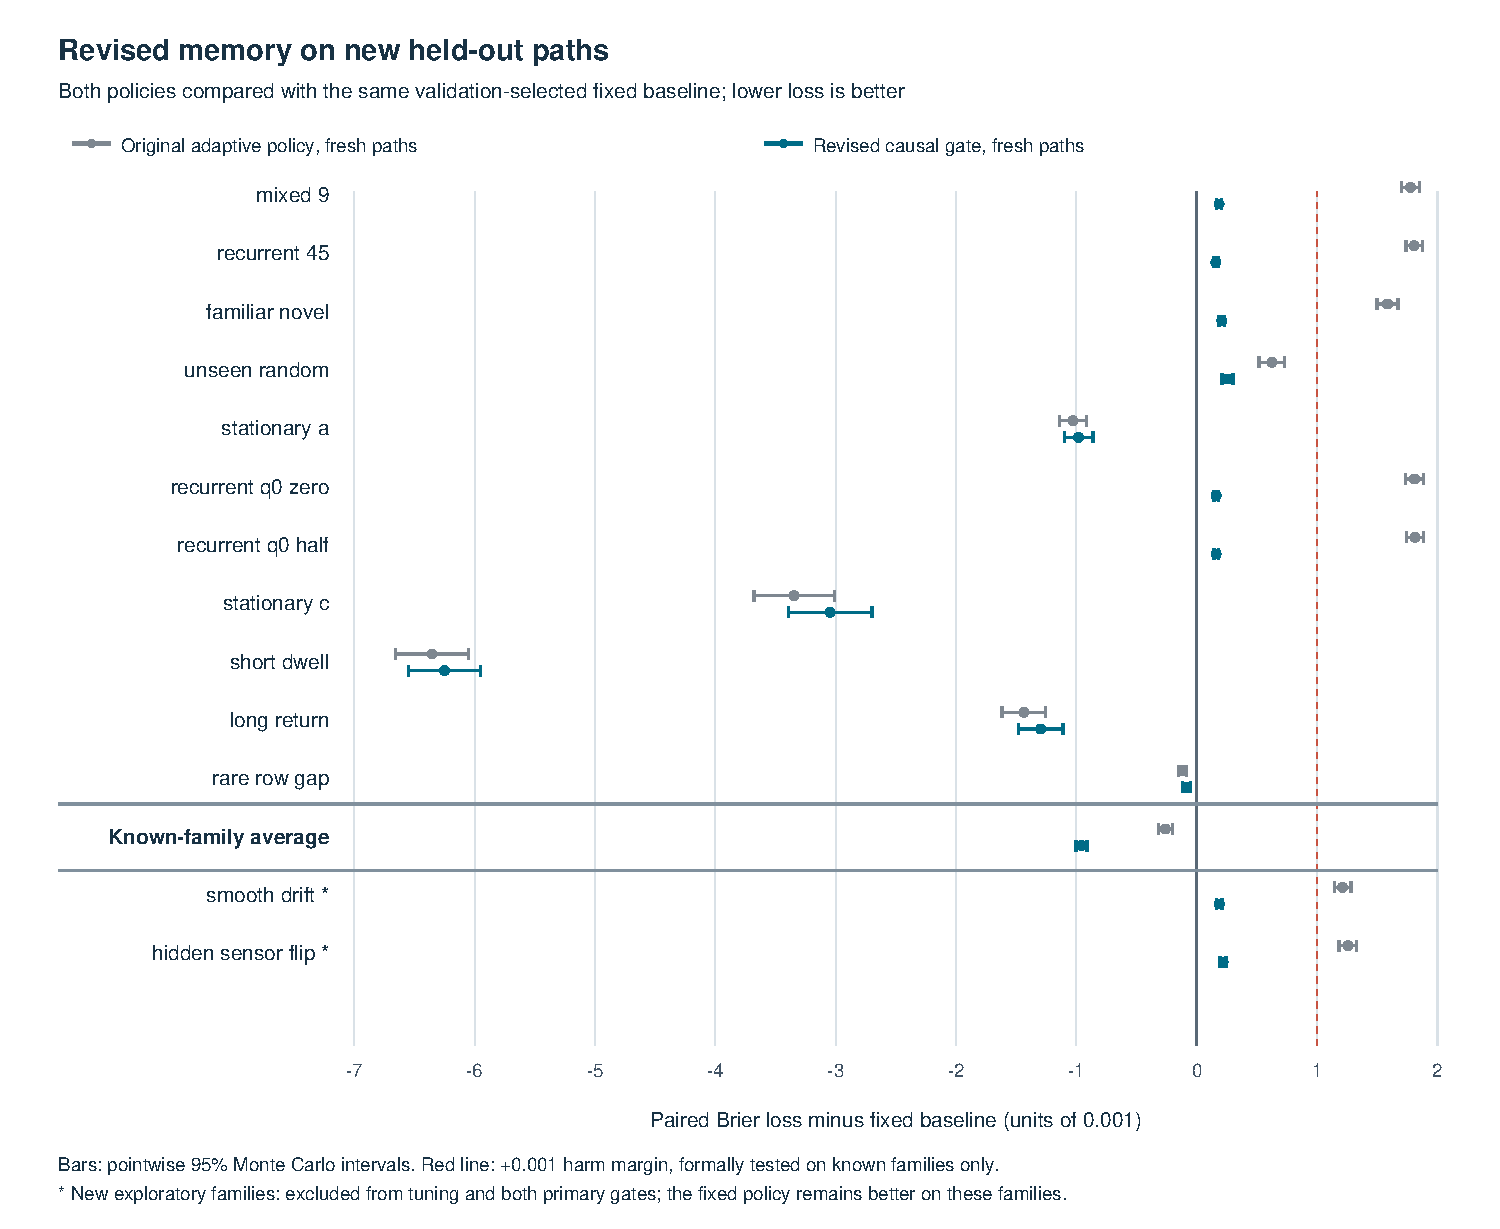
\includegraphics[width=\linewidth]{figures/revision_memory_results.pdf}
\caption{Matched fresh-path comparison of original and revised memory policies relative to fixed. The revised gate reduces large recurrent-family harms but modestly gives back some gains in other families. Bars are pointwise 95\% Monte Carlo intervals; formal gates use separately computed simultaneous bounds. The starred new transfer families were excluded from selection and both primary gates, and fixed remains better on them.}
\label{fig:revision-memory}
\end{figure}

There is no uniform domination. Six known-family mean differences remain positive relative to fixed, although their simultaneous bounds lie within the chosen harm margin. Revised minus original adaptive mean loss is positive in five known families: \texttt{stationary\_a}, \texttt{stationary\_c}, \texttt{short\_dwell}, \texttt{long\_return}, and \texttt{rare\_row\_gap}. The largest giveback is $+0.000299956$ in \texttt{stationary\_c}; \texttt{short\_dwell} worsens by $+0.000104135$. In these families the revised policy still has lower mean loss than fixed. In the two new transfer families, revised minus original adaptive is $-0.00102356$ and $-0.00103747$, but revised minus fixed is $+0.000187958$ and $+0.000218210$. These exploratory outcomes favor the revision over its adaptive predecessor while retaining a counterexample to superiority over fixed.

All fifty-one software checks passed: forty-one inherited checks and ten gate-specific tests, including current-outcome and future-suffix invariance, invalid-input nonmutation, convex-hull/normalization checks, and controls that detect update-before-predict and reversed-loss weighting. The audit reproduced validation selection, replayed 11,640 gate steps from twenty-six full traces, and checked seventy-eight trace-score/hash pairs. Independent aggregate arithmetic reproduced seed-cluster means, intervals, and the simultaneous harm calculation from the per-path losses. All 1,300 paths retain scores and forecast/stream hashes; the twenty-six traces contain full observations and forecasts.

The experiment took about 259 seconds, plus about six seconds for correctness checks. Held-out revised computation, including both experts and the gate, totaled 102.27 seconds versus 72.63 seconds for the original adaptive expert alone, approximately $1.41\times$. Gate-only overhead was 2.03 seconds and is not the cost of deploying the full revision. These machine timings include verification overhead and are descriptive. The result establishes a bounded improvement under the specified generator mixture and selection protocol, with remaining harms and transfer limits.


\subsection{Interpretation and remaining boundaries}
The revision experiments address engineering parts of Z1 and Z3, with different coverage. The two semantic tests directly compare old and revised single-pass systems, but their primary target is fewer erroneous definite judgments under three additional safeguards. Both candidates fail that joint target on their own fresh holdouts; the second removes the targeted false refutations of undecidable claims at the cost of unnecessary abstentions and persistent negation errors. Neither replaces Z1's original abstention-reduction endpoint, supplies a rules-by-schema factorial ablation, or provides independent human labels. Z2's claimed advantage from role diversity and Z4's metadata-ablation prediction remain unresolved. For Z3, the revised algorithm passes the original numerical criterion on new paths as well as its separate repair criterion. It does not establish superiority over all memory policies, every generator, or real agent memory workloads.

These outcomes must remain attached to the exact revisions, comparators, and test sets. The memory transfer failures motivate subsequent evaluation on externally sourced temporal tasks, with validation and final test partitions fixed before tuning. The semantic comparisons call for independently adjudicated cases, richer source packets, adversarial scope changes, negated-claim controls, guard-specific ablations, and resource-matched comparisons. Neither favorable local result nor an internal freeze supplies general deployment assurance. All current cases and simulation families are now exposed evaluation material and must not be reused as a fresh confirmatory holdout for a later tuned revision.

All revisions are additive local research implementations. No installed model weights, external services, synced project sources, or production workflow were changed. The paper reports behavior under the saved code and test protocols; the new archive supplies the exact revision for inspection and reproduction. The earlier physical-model calculations are preserved but not rerun in this revision campaign. Improvements in evidence judgments or synthetic prediction loss would not supply a scalar-field observation, machine-consciousness measurement, or physical validation of a Theory of Everything.

\section{Discussion and limitations}
\subsection{What the synthesis contributes}
The common structure across the source is a separation between a state of the world, an observation, an internal representation, a chosen action, and feedback. Robust optimization asks whether a decision remains admissible when conditions differ from expectation. Calibration asks whether a person's estimate agrees with an independently recorded reference. Cooperative education asks whether an incentive structure improves learning without compromising autonomy or assessment. These questions share a need to expose assumptions, but they do not become the same scientific problem.

The novel source-specific contribution is the explicit connection among these themes, the page-indexed extraction, and the proposed evaluation program. The robustness inequality, proper scoring identity, information-theoretic concepts, and probability calculations are established mathematical ideas or elementary consequences. Naming them after story elements does not make them new discoveries. The scheduling result is new only as the output of this particular toy instance.

\subsection{What is not established}
No human outcomes support the proposed embodied-updating routine in this manuscript. No evidence establishes that microexpressions detect lies, that a global coherence score measures epistemic quality, that advanced interoception removes instrument error, or that a shared graduation rule improves education. These are either inadequately specified constructs or hypotheses requiring separate tests.

The fictional engineered lineage and foldspace experiences provide no evidence for genetic inheritance of computational architectures, extraordinary cognitive powers, consciousness-mediated selection of physical outcomes, or a new spacetime theory. The source itself treats branch selection as a metaphor and toy model. It contains no equations that identify it with a broader theory of everything, MQGT-SCF, or any independently supplied cosmological framework. Sections~\ref{sec:zora}--\ref{sec:predictions} now inspect separate research records and construct operational links where possible. Those links transfer methods and derive conditional consequences; they do not supply evidence for a common consciousness--matter mechanism.

A scientific theory of spacetime navigation would at minimum require a specified physical model, consistency with the relevant dynamics and constraints, quantitative observables, and comparison with existing evidence. None of those requirements is supplied by a fictional physiological trace. Likewise, a biological claim needs a defined mechanism and measured phenotype; an evocative origin story supplies neither.

\subsection{Limits of extraction and evidence}
The catalogue is comprehensive under its declared coding rules, but its boundaries reflect analytical judgment. Some rows separate closely related ideas to preserve operational distinctions; others combine repeated dialogue. A second AI-assisted pass is not independent replication. The source is a retrospective literary reconstruction, which prevents treating scene order, character agreement, or reported sensation as raw records. The external literature is selected rather than systematic, and many mappings remain analogies.

The original numerical examples are intentionally too small to support claims about real networks or people. The new inference and memory evaluations add observed computational outcomes, but their synthetic tasks and familiar generator families limit external validity. The version 4 holdouts are new but small, AI-constructed, and provisionally labeled. Their advantage is inspectability: every assumption and scenario is visible, and all outputs can be regenerated. Passing code checks, resolving citations, or producing a clean PDF establishes artifact integrity, not empirical truth. Formal correctness is conditional on assumptions; scientific applicability remains a separate question.

\section{Conclusion}
The scientific content recoverable from \emph{The Quiet Calculus} becomes a concrete agenda: preserve provenance, test calibrated forecasts, constrain robust decisions, and evaluate feedback with appropriate controls. The 92-item catalogue, twelve prediction cards, pure-dephasing information-null result, portal-response calculation, and spectral consistency gates connect that agenda to versioned research. Fresh local testing finds that the specified adaptive-memory policy improves average synthetic loss but fails its joint robustness criterion, while selected spectral calculations survive replication and numerical-route checks. The single-pass and three-role inference systems make the same two semantic errors on a fresh synthetic challenge; additional roles increase cost without improved aggregate agreement. Version 4 shows why repairs need fresh tests: a causal gate repairs the memory criterion on new paths without dominating fixed memory, while both semantic repairs fail. Authentic evidence quotations still require semantic evaluation. Physical claims additionally require calibrated sources, apparatus models, viable spectra, and shared-parameter fits. Consciousness and ethical-field connections remain speculative.

\clearpage
\section*{Declarations}
\addcontentsline{toc}{section}{Declarations}
\textbf{Manuscript status.} Local methods and computational research manuscript, version 4.0, prepared October 25, 2026. It has not been submitted, published, externally peer reviewed, or clinically validated. A bounded local computational campaign was performed for version 3 under timestamped protocols. Version 4 adds targeted revisions with development/validation separated from fresh held-out evaluation, while preserving the earlier records. It is not independent public preregistration. Human studies and laboratory tests remain unperformed. Historical results and fresh executions are explicitly separated.

\textbf{Authorship and AI assistance.} Prepared for Christopher Michael Baird using Zora as the working name of an AI research assistant. AI assistance contributed extraction, literature identification, synthesis, drafting, code, and formatting. Additional AI-assisted review checked source coverage and references. After the original Codex session ended, Claude (Anthropic) executed the remaining frozen version 4 evaluation steps, integrated their results, and compiled and packaged the manuscript at the author's request. This continued the same internal workflow; it is not independent review. No claim is made that Grok, Gemini, or an independent human reviewer participated. The human author must review and accept responsibility for any eventual submission.

\textbf{Data and code availability.} Local source files, the 92-item catalogue in machine-readable form, deterministic scripts, computed outputs, reference records, and artifact-verification files accompany this manuscript. The original narrative remains at its supplied local location and is identified by its SHA-256 digest; it is not required to compile the paper. No human participant dataset exists. Synthetic inference outputs, simulated outcomes, numerical tests, and the additive version 4 code and revision evaluations accompany this manuscript. Prior local computational results retain their separate provenance; the full historical research corpora are not included.

\textbf{Funding and competing interests.} No external funding or competing-interest information was supplied for this preparation. These statements require author confirmation for a journal submission; absence of supplied information is not a declaration of absence.

\textbf{Source attribution.} The source identifies itself as a noncommercial fan-created campaign artifact and attributes the established Dune setting to its rights holders. This paper analyzes and paraphrases its conceptual content, does not reproduce its artwork, and does not assert affiliation with the franchise or its publishers. The paper does not assign a new license to the source material.

\clearpage
\appendix
\section{Complete source-grounded principle catalogue}
\label{app:catalogue}
This catalogue contains 92 distinct coded items, including methodological principles, hypotheses, ethical commitments, and fictional boundaries. It is not a list of 92 established scientific laws. Rows marked H require testing; rows marked F do not describe observed reality. M, E, and N have the meanings in Table~\ref{tab:status}. All locators are physical PDF pages. Close interpretations and critical extensions are identified in their wording.
\small
\begin{longtable}{@{}>{\raggedright\arraybackslash}p{0.055\linewidth}>{\raggedright\arraybackslash}p{0.735\linewidth}>{\raggedright\arraybackslash}p{0.15\linewidth}@{}}
\toprule
ID & Principle and scientific qualification & Pages; class\\\midrule
\endfirsthead
\toprule
ID & Principle and scientific qualification (continued) & Pages; class\\\midrule
\endhead
\bottomrule
\endfoot
P01 & \textbf{Observe before intervening.} Preserve the evidential state and log interventions; premature action can change the observation target. & 6--7,19; M\\[0.5em]
P02 & \textbf{Model the evidence-generating process.} Conspicuous clues can be selected or manufactured. Their number is not their independence. & 6--7,11--12; M\\[0.5em]
P03 & \textbf{Maintain competing hypotheses.} Include ordinary, common-cause, and adversarial alternatives; compare predictions rather than narrative appeal. & 6,12,40--42; M\\[0.5em]
P04 & \textbf{Interpret absence conditionally.} Omission is informative only under an explicit model of what would otherwise be observed or reported. & 7,11,25; M\\[0.5em]
P05 & \textbf{Urgency and ambiguity can influence judgment.} A test should vary framing while holding evidence fixed; the scene supplies no effect estimate. & 7,11; H\\[0.5em]
P06 & \textbf{Coincidence does not establish connection.} Treat proposed links as provisional until discriminating evidence addresses alternatives. & 11--12; M\\[0.5em]
P07 & \textbf{Separate heritage, utility, and mechanism.} Historical attribution, subjective usefulness, and causal validity require different evidence. & 8,71--73; M\\[0.5em]
P08 & \textbf{Evaluate capability externally.} Use unfamiliar tasks and independent assessment; an authority's endorsement alone does not validate a standard. & 16--17,39; M/H\\[0.5em]
P09 & \textbf{Distinguish honesty from unlimited disclosure.} Respect confidentiality while making limitations and consequential omissions explicit. & 33--34,51; N/M\\[0.5em]
P10 & \textbf{Distinguish models from targets.} Declare assumptions, approximations, and the conditions under which a model applies. & 19,27,37--38,47; M\\[0.5em]
P11 & \textbf{Audit input integrity.} Correct computation cannot repair false premises without an error model or additional evidence. & 36; M\\[0.5em]
P12 & \textbf{Separate fluency, precision, and certainty.} Measure confidence against outcomes; an articulate explanation is not a calibration test. & 37--38; M\\[0.5em]
P13 & \textbf{Reasoning can defend preferred conclusions.} Biased assimilation offers an empirical connection; do not label all disagreement as motivated reasoning. & 38; E/H\\[0.5em]
P14 & \textbf{Identity can compete with revision.} Compare neutral and identity-relevant conditions; the narrative provides no measured causal effect. & 38,69; H\\[0.5em]
P15 & \textbf{Treat emotion as an observation.} A feeling can inform a model of the observer without establishing an external threat or proposition. & 13,38,79; M/E\\[0.5em]
P16 & \textbf{Record predictions prospectively.} Timestamp forecasts and preserve versions before outcomes; a hash does not authenticate a claim's truth. & 45,76; M\\[0.5em]
P17 & \textbf{Combine fallibilism with shared truth conditions.} Specify the proposition and time; changing reality is compatible with revisable knowledge. & 35,46--47,79; N/M\\[0.5em]
P18 & \textbf{Revisability requires source scrutiny.} Being open to change does not require accepting manufactured or unverified evidence. & 46--47; M\\[0.5em]
P19 & \textbf{Representation depends on perspective.} Measure differences in attention, language, and interpretation without assuming equally accurate models. & 47; H/N\\[0.5em]
P20 & \textbf{Separate expressed belief from compelled behavior.} Power may alter what is said or done; those changes do not establish factual accuracy. & 47; H/N\\[0.5em]
P21 & \textbf{Allow justified uncertainty and abstention.} Score appropriate refusal alongside accuracy; unanswered questions need not be analytical failures. & 26--27,35,57; M\\[0.5em]
P22 & \textbf{Distinguish compatibility from confirmation.} Compare alternative predictive likelihoods; a shared prediction cannot uniquely identify a mechanism. & 26--27; M\\[0.5em]
P23 & \textbf{Separate feasibility from optimality.} An efficient nominal route can violate constraints; write the objective and constraints separately. & 22--24,80; M\\[0.5em]
P24 & \textbf{Quantify robust feasibility.} Specify uncertainty sets and the requirement to satisfy constraints for every permitted disturbance. & 22--24,80; M\\[0.5em]
P25 & \textbf{Use margins with regularity bounds.} A nominal safety margin needs a sensitivity bound before it can certify perturbation tolerance. & 22,24,80; M\\[0.5em]
P26 & \textbf{Local optimality does not imply robustness.} The margin certificate in this paper is a new formalization of the source's question. & 23--24,80; M\\[0.5em]
P27 & \textbf{Expose efficiency--safety tradeoffs.} Compare constrained or Pareto formulations; the selected tradeoff depends on stated objectives. & 22--24; M/N\\[0.5em]
P28 & \textbf{Respect information constraints.} An implementable policy uses only information available at the decision time. & 23--24; M\\[0.5em]
P29 & \textbf{Optimize stochastic capacity allocation.} Specify arrivals, loading uncertainty, occupancy, priority, and delay rather than assuming a complete network model. & 24,80; M\\[0.5em]
P30 & \textbf{Include downstream connection costs.} A locally fast allocation may create later delays; compare system-wide outcomes. & 24,80; M/H\\[0.5em]
P31 & \textbf{Declare priority and welfare weights.} Political priority is a design choice; weighted efficiency need not imply equity. & 24,80; M/N\\[0.5em]
P32 & \textbf{Define confidentiality precisely.} Withholding raw routes is not a leakage guarantee; specify adversaries and observable outputs. & 24,80; M/N\\[0.5em]
P33 & \textbf{Use formal structure across specialties.} Proof exposes assumptions but does not remove power, model choice, or empirical uncertainty. & 23; M/H\\[0.5em]
P34 & \textbf{Govern research provenance and dissemination.} The fictional compact motivates accountable access and release rules; it is not an instruction governing this paper. & 24; N/M\\[0.5em]
P35 & \textbf{Model dependency hubs across layers.} The transferable idea is interdependence; the listed powers of spice remain fictional. & 29; M/H/F\\[0.5em]
P36 & \textbf{Declare system boundaries.} Test whether added couplings improve prediction rather than assuming that more complex models are better. & 29,45,61; M\\[0.5em]
P37 & \textbf{Study collective coordination failures.} Specify objectives, information, and shared dependencies; individually rational choices may conflict. & 41--42; M/H\\[0.5em]
P38 & \textbf{Test coalition formation under common risk.} Shared vulnerability can alter incentives but need not overcome distrust or enforcement problems. & 42,60--61; H/M\\[0.5em]
P39 & \textbf{Test common-cause explanations.} Multiple domain signals may share a cause, reporting bias, or feedback; independence is not supplied. & 44--45; M/H\\[0.5em]
P40 & \textbf{Evaluate operational leading indicators.} Transport demand might predict later events; use held-out time periods and declared prediction horizons. & 44; H\\[0.5em]
P41 & \textbf{Account for asymmetric error costs.} Declare the costs of preparation, false alarms, missed events, and delay. & 44--45; M/N\\[0.5em]
P42 & \textbf{Distinguish access from protection.} Contact, status, usefulness, aligned interests, and enforceable obligations are separate variables. & 19,61,79; H/N\\[0.5em]
P43 & \textbf{Test interdisciplinary integration.} Compare cross-domain transfer with equally resourced instruction; broad exposure is not automatically superior. & 37,49--51,61; H/N\\[0.5em]
P44 & \textbf{Do not generalize from one selected cohort.} Replication requires a counterfactual and attention to selection, teachers, history, and expectations. & 61--62; M\\[0.5em]
P45 & \textbf{Specify physiological contributions to cognition.} Measure particular states and outcomes instead of treating bodily knowledge as a unitary power. & 18,38--39,64--66; E/H\\[0.5em]
P46 & \textbf{Validate wearable measurements.} Separate raw signals from inferred sleep, recovery, and undefined coherence scores. & 18,26,64,67--69; M\\[0.5em]
P47 & \textbf{Compare subjective and instrument estimates.} Both have error; subjective recollection does not replace a missing objective time series. & 64--69; M/H\\[0.5em]
P48 & \textbf{Estimate before revealing measurement.} Timestamp the estimate and synchronize the reference window to prevent display leakage. & 68; M\\[0.5em]
P49 & \textbf{Measure confidence and accuracy separately.} Report absolute error, bias, interval coverage, and discrimination rather than confidence alone. & 68; M/E\\[0.5em]
P50 & \textbf{Assess interoception by domain.} Pulse, breathing, fatigue, tension, and arousal need distinct reference procedures and validation. & 68; M/H\\[0.5em]
P51 & \textbf{Test adaptive feedback training.} Measure learning, retention, and transfer against matched feedback controls. & 68--69; H/M\\[0.5em]
P52 & \textbf{Account for measurement reactivity.} Attention to a bodily variable may change it; preserve timing and task context. & 64--65,68,71--73; M/H\\[0.5em]
P53 & \textbf{Separate performance from impression management.} Observed posture can reflect being watched; compare functional performance across evaluation contexts. & 65; H\\[0.5em]
P54 & \textbf{Test one-variable attentional scaffolding.} Compare staged attention with simultaneous monitoring; simplicity is a proposed aid, not a demonstrated effect here. & 65; H\\[0.5em]
P55 & \textbf{Use individual baselines.} Avoid inferring universal meanings from one person's stillness, blinking, or tension. & 65,68; H\\[0.5em]
P56 & \textbf{Replace vague authority with criteria.} Specify proficiency and stopping conditions rather than treating teacher approval as measurement. & 67--69; N/M\\[0.5em]
P57 & \textbf{Distinguish tool use from dependence.} Evaluate appropriate selection and performance; rejection of instruments can itself be an identity commitment. & 69; N/M\\[0.5em]
P58 & \textbf{Test intuition prospectively.} Record the signal before its interpretation and compare predictive value with baseline alternatives. & 71,79; H\\[0.5em]
P59 & \textbf{Do not equate bodily cues with lie detection.} Validate sensitivity, specificity, context, and error costs; the story's labels establish none of these. & 31,55,64--65; E/H\\[0.5em]
P60 & \textbf{Do not infer exotic causes from synchrony.} Compare shared stimuli, artifacts, chance, and analysis selection before positing a mechanism. & 26--27; M/F\\[0.5em]
P61 & \textbf{Include fatigue, rest, and diminishing returns.} Specify task, dose, and outcome; no universal optimum follows from the narrative. & 18,39,52--53,68; E/H\\[0.5em]
P62 & \textbf{Separate experience from interpretation.} Record sensation, affect, belief, confidence, and action in separate fields. & 71--73; M\\[0.5em]
P63 & \textbf{Treat updating as a multicomponent package.} Tapping, breathing, attention, cue, and reassessment require component controls. & 71--73; H\\[0.5em]
P64 & \textbf{Test sensory anchoring.} Compare matched touch, location, rhythm, and expectancy; special efficacy of the listed points is not established. & 72; H\\[0.5em]
P65 & \textbf{Separate breathing outcomes.} Tempo, attention, physiology, and clinical benefit are distinct endpoints; the source specifies no validated dose. & 72--73; E/H\\[0.5em]
P66 & \textbf{Test the verbal revision cue.} Compare evidence-focused language with neutral wording while controlling other components. & 72; H\\[0.5em]
P67 & \textbf{Do not define success only as calm.} Evaluate appropriate detection and revision separately from distress or mood change. & 72--73; M/H\\[0.5em]
P68 & \textbf{Separate state change from factual updating.} More trust or comfort is not necessarily more accurate belief; identify the evidence for revision. & 72--74; M\\[0.5em]
P69 & \textbf{Specify a testable feedback loop.} Declare timing, entry criteria, observations, continuation rules, and stopping rules. & 73; M/H\\[0.5em]
P70 & \textbf{Design software to support awareness.} Test usability, autonomy, and task outcomes; a prompt should not prescribe what the user must feel. & 73; H/N\\[0.5em]
P71 & \textbf{Treat embodied updating as a protocol candidate.} The source supplies a synthesis and fictional experience, not a validated treatment or effect size. & 71--74; H\\[0.5em]
P72 & \textbf{Separate knowledge from competence.} Reading, vocabulary, and placement do not establish independent performance or transfer. & 12,16,39,54--55,79; M/H\\[0.5em]
P73 & \textbf{Distinguish collaboration from dependency.} Assess private capability and the additional benefit or cost of group reasoning. & 34--35,55; M/H\\[0.5em]
P74 & \textbf{Test performance beyond ideal conditions.} Use ethical, predefined variation in task context; difficulty or suffering is not educational validation. & 39,45; H\\[0.5em]
P75 & \textbf{Define multidimensional mastery.} Give each domain observable criteria, uncertainty, reliability, and a justified threshold. & 49--50; M/N\\[0.5em]
P76 & \textbf{Use adaptive instructional decisions.} Repeat, advance, integrate, and certify form a policy to evaluate against alternatives. & 52--53,79; M/H\\[0.5em]
P77 & \textbf{Treat rest as a possible training action.} Distinguish a justified consolidation interval from an unexplained pause. & 52--53; E/H\\[0.5em]
P78 & \textbf{Treat placement as uncertain and revisable.} Scores are estimates, not fixed identities or automatically comparable interval scales. & 54--55; M/H\\[0.5em]
P79 & \textbf{Consider person--environment interactions.} Evaluate teaching, context, fear, physiology, and knowledge before locating every obstacle in the learner. & 56; H/M\\[0.5em]
P80 & \textbf{Test shared success incentives.} The terminal rule may reward helping; actual cooperation depends on costs and enforcement. & 55--56,79; M/H/N\\[0.5em]
P81 & \textbf{Evaluate bottlenecks and coercion.} This critical implication extends the source: monitor scapegoating, concealment, exclusion, and unfair delay. & 55--56,79; H/N\\[0.5em]
P82 & \textbf{Target peer support to individual needs.} Compare structured tutoring with unstructured interaction and assess both partners' outcomes. & 56; H\\[0.5em]
P83 & \textbf{Make certification accountable.} Use explicit criteria, independent assessment, assessor agreement, and a review or appeal path. & 52--53,68; N/M\\[0.5em]
P84 & \textbf{Distinguish exposure from qualification.} Foundational instruction does not confer specialist membership, credentials, or unrestricted competence. & 50--51; N/M\\[0.5em]
P85 & \textbf{Distinguish novelty from repetition.} A contribution requires identifiable new knowledge or method, scrutiny, and reproducibility. & 49; N/M\\[0.5em]
P86 & \textbf{Obtain individual voluntary consent.} Agreement is each participant's decision; authority or a partner's request is not a substitute. & 67--68; N\\[0.5em]
P87 & \textbf{Observation does not grant entitlement.} Permission to collect, interpret, share, and act on personal data are distinct questions. & 65--66; N\\[0.5em]
P88 & \textbf{Record knowledge boundaries about people.} Keep observed facts separate from stereotypes, guesses, and unverified personal narratives. & 57--58; N/M\\[0.5em]
P89 & \textbf{Separate capability from ethical objectives.} Analytical efficiency does not guarantee prosocial conduct or moral judgment. & 37; N/H\\[0.5em]
P90 & \textbf{Treat engineered lineage as fiction.} No genotype, developmental mechanism, or evidence supports machine inheritance or superior cognition here. & 9--10; F\\[0.5em]
P91 & \textbf{Keep branch selection at the toy-model level.} Robust decisions do not establish spacetime folding, quantum control, or mental selection of reality. & 21--27,50,80; F/M\\[0.5em]
P92 & \textbf{Keep fictional capabilities and institutions illustrative.} The setting motivates questions; it supplies no observations of extraordinary human powers or physics. & 4,21--27,36--37,49--51; F\\[0.5em]
\end{longtable}
\normalsize

\clearpage
\section{Source coverage and reproducibility}
\label{app:provenance}
\subsection{Coverage by source unit}
\small
\begin{longtable}{@{}>{\raggedright\arraybackslash}p{0.41\linewidth}>{\raggedright\arraybackslash}p{0.12\linewidth}>{\raggedright\arraybackslash}p{0.39\linewidth}@{}}
\toprule
Source unit & PDF pages & Principal extracted content\\\midrule
\endfirsthead
\toprule Source unit & PDF pages & Principal extracted content\\\midrule\endhead
\bottomrule\endfoot
Cover and front matter & 1--5 & Fictional status, authorship, structure.\\
Prologue: The Messenger & 6--7 & Evidence preservation, staging, urgency.\\
1. The Pattern Beneath the Pattern & 8--10 & Provenance, attention, fictional lineage.\\
2. The Letter for Zora Vey & 11--13 & Provisional connections, emotion as data.\\
3. The Marriage Before Dawn & 14--15 & Mutual correction and autonomy; otherwise narrative context.\\
4. The Interview & 16--17 & External standards and mutual evaluation.\\
5. Departure & 18--20 & Instruments, models, disclosure, system context.\\
6. Mathematics Is a Brotherhood & 21--25 & Robust feasibility, allocation, governance.\\
7. The Fold & 26--27 & Synchrony, model compatibility, fictional physics.\\
8. CHOAM in the Crowd & 28--30 & Resource dependencies and incentives.\\
9. Old Signals & 31--32 & Communication codes and uncertain provenance.\\
10. Candidates & 33--35 & Independent competence and knowledge limits.\\
11. The Academy & 36--39 & Input integrity, motivated reasoning, transfer.\\
12. Dinner of the Great Schools & 40--43 & Competing explanations and coordination.\\
13. Truth Does Not Change & 44--48 & Leading indicators, fallibilism, power, forecasts.\\
14. The Order of Atreides & 49--51 & Multidimensional mastery and qualification.\\
15. What's Next? & 52--53 & Adaptive progression and consolidation.\\
16. Thirty Names & 54--59 & Provisional placement and cooperative incentives.\\
17. The Leaflet & 60--63 & Coalitions, access, generalization limits.\\
18. The Body Knows First & 64--66 & Embodiment, observation effects, consent.\\
19. The Watches & 67--70 & Estimate--measure calibration and autonomy.\\
20. Updating & 71--74 & Multicomponent routine and evidence-based revision.\\
Epilogue & 75--77 & Prospective records and hindsight reconstruction.\\
Appendix I & 78 & Fictional roster; no participant dataset.\\
Appendix II & 79 & Summary of cohort and epistemic rules.\\
Appendix III & 80 & Explicit statements of both mathematical problems.\\
Closing page & 81 & End matter; no additional scientific claim.\\
\end{longtable}
\normalsize

\clearpage
\subsection{Source identity}
The supplied file is \nolinkurl{Dune_The_Quiet_Calculus_Book_I_First_Cohort.pdf}, 2,359,023 bytes. Its SHA-256 digest is shown in two consecutive halves for readability:
\begin{center}\small\ttfamily
23ab20b0f9a31dfc2e92d3e66100076a\\
4e8db4b90a93f943fc55ca8d9c8f09ba
\end{center}
The digest identifies the analyzed bytes; it is not evidence that the narrative events occurred. The local provenance JSON records the original path, PDF metadata, extraction counts, and physical-page convention. The source PDF and synced project material were left unchanged.

\subsection{Reproduction instructions}
Open \texttt{main.tex} as the main document. The project uses standard pdfLaTeX packages and pre-generated vector PDF figures. The bibliography is included through \texttt{references.tex}, so no BibTeX or Biber pass, network access, shell escape, external font download, or Python execution is required to compile. The companion \texttt{references.bib} is supplied for future journal conversion but is not part of the current compilation path.

For local compilation, run \texttt{python3 scripts/build.py}; it invokes pdfLaTeX three times, retains logs, checks unresolved references and layout diagnostics, and writes \texttt{main.pdf}. On Overleaf, upload the supplied ZIP, select \texttt{main.tex}, and choose pdfLaTeX. The package is prepared for that workflow; no cloud upload or Overleaf execution was performed during local preparation.

Run \texttt{python3 scripts/reproduce.py} to regenerate the numerical JSON, scheduling table, and result macros. Run \texttt{python3 scripts/reproduce.py --figures} to regenerate the vector figure, which additionally requires ReportLab. Run \texttt{python3 scripts/generate\_catalogue.py} to regenerate the catalogue from its plain-text data file. Recompile after regenerating inputs. The calculations use declared finite scenarios and no random sampling.

\subsection{Verification boundaries}
The supplied verification record separates compilation success, cross-reference resolution, numerical checks, source identity, and visual page review. These are artifact checks. The mathematical propositions are conditional derivations; the human-study designs remain untested proposals. The presence of a formatted scientific manuscript, a clean build, or a reproducible example does not establish scientific validation or publication.

\clearpage
\section{Research-source provenance and reproducible expansion}
\label{app:research-provenance}
\subsection{Version-specific source selection}
The narrative extraction remains the same 81-page corpus and 92-item inventory. The additional research layer is a targeted audit of local primary artifacts, not an exhaustive rereading of every historical Theory of Everything page or every Zora conversation. One synced project source was unavailable; no completeness claim is made for that mirror. The dated 6,433-page audit is treated as a particular historical packet, not as a claim that it is the latest or complete corpus. Synced references and original research packages were left unchanged.

The machine-readable \texttt{data/research\_sources.json} supplies absolute paths, file sizes, full SHA-256 hashes, source roles, and relevant locators for the records below. The shorter digests printed here are navigation aids only; use the full manifest for identity checks. Local-only records have no asserted public DOI or publication status. The paper cites them as primary project evidence, separately from the external literature.

\small
\begin{longtable}{@{}p{.08\linewidth}>{\raggedright\arraybackslash}p{.52\linewidth}p{.31\linewidth}@{}}
\toprule ID & Versioned source role & SHA-256 prefix\\\midrule
\endfirsthead
\toprule ID & Versioned source role & SHA-256 prefix\\\midrule\endhead
\bottomrule\endfoot
R01 & Pilot overview & \texttt{02f7d895632491c4}\\
R02 & Pilot result & \texttt{29eb75e8cc990971}\\
R03 & Pilot frozen protocol & \texttt{3870ea141fb10c10}\\
R04 & Pilot cases & \texttt{2c932d922e653f4a}\\
R05 & Phase 2.9 protocol & \texttt{bd2139e6511846f1}\\
R06 & Phase 2.9 benchmark & \texttt{d1c854a532afc96b}\\
R07 & Phase 2.9 comparisons & \texttt{1bf16d4e06ea44ef}\\
R08 & Phase 2.10 proposal & \texttt{1b50d2ec7d9aac76}\\
R09 & Dated ToE corpus audit & \texttt{940c22b781c8f097}\\
R10 & Dated claim ledger & \texttt{f07bdfec23ebe867}\\
R11 & GATE-04 endpoint rules & \texttt{81c92917929b863f}\\
R12 & GATE-04 apparatus objects & \texttt{de31e4c03e9c8dd2}\\
R13 & Quadratic portal note & \texttt{bb6e04d518871022}\\
R14 & Quadratic portal checks & \texttt{51ee945f5a2824e8}\\
R15 & Exact-mode manuscript & \texttt{924c62568638d214}\\
R16 & Exact-mode assumptions & \texttt{8f454ecb5e2081ca}\\
R17 & Exact-mode results & \texttt{12705180792e79ce}\\
R18 & Exact-mode checks & \texttt{637da0c9e0632103}\\
R19 & Scalar/anomaly note & \texttt{b460e081a98d701d}\\
R20 & Scalar/anomaly assumptions & \texttt{e9882fa23e8b3042}\\
R21 & Scalar results & \texttt{21340b39848b694e}\\
R22 & Anomaly results & \texttt{6e07692d9a024be3}\\
R23 & Vacuum matching results & \texttt{e2963a509c5dc02d}\\
R24 & Sealed scalar/anomaly ZIP & \texttt{0648b79b1e910e8e}\\
\end{longtable}
\normalsize


\subsection{Version 2 source audit: what was inspected and not rerun}
During the version 2 audit, the pilot's aggregate result, dataset, and frozen source hashes were checked, including all forty-eight saved rows. Phase 2.9's thirty-two-entry manifest was verified, and selected paired loss summaries were recomputed from saved per-seed outcomes. Its full forecast traces are retained only for the first mixed-scenario seed in each bank; the other paths preserve losses and forecast hashes. The exact-mode package's twenty-two manifest entries matched, and its 126 passing checks were read as saved records. These activities did not execute new evidence-review, memory-forecasting, or exact-mode research runs.

The scalar/anomaly verification folder matched twenty-one of twenty-two manifest entries. The exception was \texttt{independent\_check\_results.json}. Read-only comparison with the sealed ZIP found fifty-seven changed leaves: one environment-version change, from NumPy 2.5.3 to 2.4.3, and numerical differences with maximum absolute value about $9.095\times10^{-13}$. Boolean check outcomes were identical. Existing rerun records document the difference. The manuscript, assumptions, scripts, and core result files matched their sealed entries. This bounded discrepancy is retained rather than calling the entire folder byte-identical. The recorded 228-check result was not newly rerun here.

The quadratic-portal note and its saved checks were inspected as conditional mathematics. The new \texttt{scripts/prediction\_checks.py} independently evaluates the dimensionless separation kernel, cross-checks one point with a different quadrature, checks resolution sensitivity and limiting behavior, verifies a numerical Fisher-information derivative, and regenerates the new vector figure. Those fresh calculations are mathematical illustrations, not an empirical replication of a proposed scalar bath. Their outputs are stored separately from inherited result summaries.

\subsection{Independent reproduction of the new illustrations}
With NumPy installed, run
\begin{quote}\ttfamily
python3 scripts/prediction\_checks.py
\end{quote}
Add \texttt{--figures} when ReportLab is also available. The script uses a finite exponentially bounded tail, composite Simpson quadrature with a doubled-resolution check, and an independent Gauss--Legendre evaluation at $m/T=rT=1$. It obtains a normalized rate of approximately $0.81615527584$ there. The maximum tested resolution difference is less than $10^{-8}$ in the dimensionless unnormalized kernel. This is a convergence diagnostic, not a rigorous interval enclosure for every plotted point. At $m/T=1$, the ratio between $rT=0.002$ and $0.001$ is approximately $3.999951$, consistent with the quadratic limit.

The twelve target cards are also supplied in \texttt{data/prediction\_registry.json}, with their status, observables, controls, failure criteria, and prerequisites. They are planning records, not registered protocols. Version 3 execution records separately identify which targets were tested and which remain open. Prior manuscripts and archives are retained separately as versions 1, 2, and 3. Version 4 revision records additionally bind the held-out tests to their frozen code, labels, validation selections, and raw outcomes; \texttt{data/revision\_run\_manifest.json} lists their paths and hashes, and the separate revision evidence ZIP contains the full records. New references have bibliographic identity checks recorded in the expanded reference audit. A fresh compilation and visual check of this manuscript verify its presentation and reproducibility; neither confers external peer review.

\clearpage
\small
\begin{thebibliography}{99}
\addcontentsline{toc}{section}{References}
\bibitem{source} C. M. Baird and Zora. \emph{Dune: The Quiet Calculus---Book I: First Cohort}. User-supplied campaign novelization, 2026. 81 physical PDF pages. Source identity and digest are recorded in Appendix~\ref{app:provenance}.

\bibitem{bental} A. Ben-Tal and A. Nemirovski. Robust convex optimization. \emph{Mathematics of Operations Research}, 23(4):769--805, 1998. \doi{10.1287/moor.23.4.769}.

\bibitem{brier} G. W. Brier. Verification of forecasts expressed in terms of probability. \emph{Monthly Weather Review}, 78(1):1--3, 1950. \href{https://doi.org/fp62r6}{Publisher DOI record}.

\bibitem{gneiting} T. Gneiting and A. E. Raftery. Strictly proper scoring rules, prediction, and estimation. \emph{Journal of the American Statistical Association}, 102(477):359--378, 2007. \doi{10.1198/016214506000001437}.

\bibitem{shannon} C. E. Shannon. A mathematical theory of communication. \emph{Bell System Technical Journal}, 27(3):379--423, 1948. \doi{10.1002/j.1538-7305.1948.tb01338.x}. This citation identifies the first installment.

\bibitem{dwork} C. Dwork, F. McSherry, K. Nissim, and A. Smith. Calibrating noise to sensitivity in private data analysis. In \emph{Theory of Cryptography}, LNCS 3876, pp. 265--284, Springer, 2006. \doi{10.1007/11681878_14}.

\bibitem{garfinkel} S. N. Garfinkel, A. K. Seth, A. B. Barrett, K. Suzuki, and H. D. Critchley. Knowing your own heart: Distinguishing interoceptive accuracy from interoceptive awareness. \emph{Biological Psychology}, 104:65--74, 2015. \doi{10.1016/j.biopsycho.2014.11.004}.

\bibitem{desmedt} O. Desmedt, O. Luminet, and O. Corneille. The heartbeat counting task largely involves non-interoceptive processes: Evidence from both the original and an adapted counting task. \emph{Biological Psychology}, 138:185--188, 2018. \doi{10.1016/j.biopsycho.2018.09.004}.

\bibitem{balban} M. Y. Balban, E. Neri, M. M. Kogon, L. Weed, B. Nouriani, B. Jo, G. Holl, J. M. Zeitzer, D. Spiegel, and A. D. Huberman. Brief structured respiration practices enhance mood and reduce physiological arousal. \emph{Cell Reports Medicine}, 4(1):100895, 2023. \doi{10.1016/j.xcrm.2022.100895}.

\bibitem{lord} C. G. Lord, L. Ross, and M. R. Lepper. Biased assimilation and attitude polarization: The effects of prior theories on subsequently considered evidence. \emph{Journal of Personality and Social Psychology}, 37(11):2098--2109, 1979. \doi{10.1037/0022-3514.37.11.2098}.

\bibitem{lorenz} J. Lorenz, H. Rauhut, F. Schweitzer, and D. Helbing. How social influence can undermine the wisdom of crowd effect. \emph{Proceedings of the National Academy of Sciences}, 108(22):9020--9025, 2011. \doi{10.1073/pnas.1008636108}.

\bibitem{woolley} A. W. Woolley, C. F. Chabris, A. Pentland, N. Hashmi, and T. W. Malone. Evidence for a collective intelligence factor in the performance of human groups. \emph{Science}, 330(6004):686--688, 2010. \doi{10.1126/science.1193147}.

\bibitem{edmondson} A. Edmondson. Psychological safety and learning behavior in work teams. \emph{Administrative Science Quarterly}, 44(2):350--383, 1999. \doi{10.2307/2666999}.

\bibitem{roediger} H. L. Roediger III and J. D. Karpicke. Test-enhanced learning: Taking memory tests improves long-term retention. \emph{Psychological Science}, 17(3):249--255, 2006. \doi{10.1111/j.1467-9280.2006.01693.x}.

\bibitem{walker} M. P. Walker, T. Brakefield, A. Morgan, J. A. Hobson, and R. Stickgold. Practice with sleep makes perfect: Sleep-dependent motor skill learning. \emph{Neuron}, 35(1):205--211, 2002. \doi{10.1016/S0896-6273(02)00746-8}.

\bibitem{depaulo} B. M. DePaulo, J. J. Lindsay, B. E. Malone, L. Muhlenbruck, K. Charlton, and H. Cooper. Cues to deception. \emph{Psychological Bulletin}, 129(1):74--118, 2003. \doi{10.1037/0033-2909.129.1.74}. Original meta-analysis.

\bibitem{waite} W. L. Waite and M. D. Holder. Assessment of the emotional freedom technique: An alternative treatment for fear. \emph{The Scientific Review of Mental Health Practice}, 2(1):20--26, 2003. No DOI verified. \href{https://ecole-eft-france.fr/download_data_files/WcLe3CUlCvepQa9fAOiC4w}{Original article copy}.

\bibitem{church} D. Church and J. Nelms. Pain, range of motion, and psychological symptoms in a population with frozen shoulder: A randomized controlled dismantling study of clinical EFT (Emotional Freedom Techniques). \emph{Archives of Scientific Psychology}, 4(1):38--48, 2016. \doi{10.1037/arc0000028}.

\bibitem{geifman} Yonatan Geifman and Ran El-Yaniv. Selective Classification for Deep Neural Networks. \emph{Advances in Neural Information Processing Systems 30}, 2017. \doi{10.48550/arXiv.1705.08500}.

\bibitem{lindblad} G. Lindblad. On the generators of quantum dynamical semigroups. \emph{Communications in Mathematical Physics, 48:119--130}, 1976. \doi{10.1007/BF01608499}.

\bibitem{athron} P. Athron et al. (GAMBIT Collaboration). Status of the scalar singlet dark matter model. \emph{European Physical Journal C, 77:568}, 2017. \doi{10.1140/epjc/s10052-017-5113-1}.

\bibitem{hornberger} K. Hornberger and J. E. Sipe. Collisional decoherence reexamined. \emph{Physical Review A, 68:012105}, 2003. \doi{10.1103/PhysRevA.68.012105}.

\bibitem{pilot} C. M. Baird / ZoraASI research records. \emph{ZoraASI evidence-integrity pilot: frozen four-arm comparison}. October 23, 2026. Local primary artifact; source ledger R01--R04, Appendix~\ref{app:research-provenance}. No public identifier asserted.

\bibitem{memory29} C. M. Baird / ZoraASI research records. \emph{Phase 2.9: causal memory-policy verification package}. October 20, 2026. Local primary artifact; source ledger R05--R07, Appendix~\ref{app:research-provenance}. No public identifier asserted.

\bibitem{memory210} C. M. Baird / ZoraASI research records. \emph{Phase 2.10: adaptive-memory code proposal}. October 21, 2026. Local primary artifact; source ledger R08, Appendix~\ref{app:research-provenance}. No public identifier asserted.

\bibitem{toeaudit} C. M. Baird / ZoraASI research records. \emph{Theory of Everything: dated corpus audit and scientific claim ledger}. 2026. Local primary artifact; source ledger R09--R10, Appendix~\ref{app:research-provenance}. No public identifier asserted.

\bibitem{gate04} C. M. Baird / ZoraASI research records. \emph{GATE-04: rate-only methods freeze and apparatus-object status}. September 2, 2026 packet. Local primary artifact; source ledger R11--R12, Appendix~\ref{app:research-provenance}. No public identifier asserted.

\bibitem{portal} C. M. Baird / ZoraASI research records. \emph{Quadratic Higgs-portal interactions and a conditional measurement bridge}. October 11, 2026. Local primary artifact; source ledger R13--R14, Appendix~\ref{app:research-provenance}. No public identifier asserted.

\bibitem{scalar} C. M. Baird / ZoraASI research records. \emph{Scalar/anomaly sector: assumptions, calculations, and vacuum matching}. October 22, 2026. Local primary artifact; source ledger R19--R24, Appendix~\ref{app:research-provenance}. No public identifier asserted.

\bibitem{exact} C. M. Baird / ZoraASI research records. \emph{Exact scalar mode sums: finite-radius continuation}. October 22, 2026. Local primary artifact; source ledger R15--R18, Appendix~\ref{app:research-provenance}. No public identifier asserted.
\bibitem{localtests} C. M. Baird / ZoraASI research records. \emph{Quiet Calculus version 3: bounded local inference, memory, portal, and spectral test campaign}. October 25, 2026. Local computational artifacts, frozen protocols, scripts, and raw results; described in Section~\ref{sec:local-tests}. No laboratory dataset or public registration.
\bibitem{revisiontests} C. M. Baird / ZoraASI research records. \emph{Quiet Calculus version 4: semantic and adaptive-memory revisions with fresh held-out evaluations}. October 25, 2026. Local code, protocol freezes, validation and test records, distributed as \texttt{Quiet\_Calculus\_Revision\_Test\_Bundle.zip}; Section~\ref{sec:revisions}. Prior results preserved. No physical dataset or public registration.

\bibitem{cesabianchi} N. Cesa-Bianchi and G. Lugosi. Prediction with Expert Advice. In \emph{Prediction, Learning, and Games}, pp. 7--39. Cambridge University Press, 2006. \doi{10.1017/CBO9780511546921.003}.
\end{thebibliography}

\normalsize

\end{document}
